\documentclass[journal]{IEEEtran}

\usepackage[utf8]{inputenc}
\usepackage[T1]{fontenc}
\usepackage{amsmath,amssymb,amsfonts}
\usepackage{amsthm}
\usepackage{graphicx}
\usepackage{booktabs}
\usepackage{array}
\usepackage{cite}
\usepackage{enumitem}
\usepackage[colorlinks=true,linkcolor=blue,citecolor=blue,urlcolor=blue]{hyperref}
\usepackage{xeCJK}
\setCJKmainfont{Heiti SC}

\newtheorem{theorem}{定理}
\newtheorem{proposition}{命题}
\newtheorem{definition}{定义}

\begin{document}

\title{面向受约束物理人机交互的行为--实现分离\\[2pt]\large（中文译本）}

\author{Yongyan~Cao%
\thanks{Y. Cao 就职于 Voryx Robotic LLC，San Jose, CA 95136, USA
(e-mail: yongyancao@gmail.com)。本文为英文原稿的中文译本，内容以英文原稿为准。}}

\maketitle

\begin{abstract}
物理人机交互软件常常把"期望行为的说明"与"受约束的实现"耦合在一起；本文把二者当作独立的两层来处理。一个\emph{行为层}提供期望的接触端口加速度 $a_k^{\mathrm{id}}=f_\theta(e_k,\dot e_k,F_{h,k})$。一个\emph{实现层}把它转换为受约束的机器人指令，并报告"期望加速度与实现加速度"之间的总误差，而不是把它隐藏在饱和之中。一个同目标的无约束反事实方案，把正则化与约束介入区分开；被控对象的实测数据则暴露出模型误差。本文实现了一个滚动时域二次规划（QP），用于实现无记忆仿射行为。改变行为只需通过 $(C_\theta,G_\theta)$ 改变目标函数系数，机器人指令变量与可行集保持不变。一项平面研究实例化了阻抗与导纳；同一个运行中的实现层在其现有速率限制下，无需重建即可接受"阻抗$\to$导纳$\to$阻抗"这样的重新指派。在一台 MuJoCo 中力矩控制的 7 自由度 Franka FR3 上，运行时在每次求解时冻结任务空间动力学，并在整个时域上强制力矩可行性。在一个持续 20~N 的推力下，它把一个经松弛处理的工作空间边界保持在约 0.1--0.2~mm 以内，而瞬时截断方式则会产生 4.4~cm（阻抗）与 4.7~cm（导纳）的越界。随后，一个降额的执行器预算激活了力矩约束：全时域强制约束把其冻结模型计划的可行性维持在 $2.1\times10^{-4}$~N$\cdot$m 以内，而一个仅约束第一步的消融方案则会规划出最多超出预算 11.329~N$\cdot$m 的方案；在实际执行的非线性被控对象上，由于二者共享同样的局部模型误差，差距会缩小，但仍然是全时域强制约束更优（0.161 对 0.380~N$\cdot$m）。这些结果是对行为--实现分离的一次聚焦的证明，而不是一个新的 MPC 或安全滤波器原理（范围界定见第~\ref{sec:scope}节）。
\end{abstract}

\begin{IEEEkeywords}
物理人机交互、行为--实现分离、机器人控制架构、预测式实现、模型预测控制、阻抗控制、导纳控制。
\end{IEEEkeywords}

\section{引言}
\label{sec:intro}

交互行为应当只说明期望的交互动力学；物理可行性应当由机器人独立地实现。

一个 pHRI 软件栈有两个概念上不同的职责：
\begin{enumerate}
\item 说明期望的交互行为；以及
\item 通过与物理机器人相容的指令实现该行为。
\end{enumerate}

\noindent\textbf{架构假设。} 我们主张上述这一通用的软件工程原则，也主张它应当成立的一个具体理由：期望的交互行为是交互状态空间中的一个陈述——位置误差、速度误差与人类作用力——而物理可行性则是机器人约束空间中的一个陈述——关节力矩、关节限位与工作空间几何。这是两类具有不同自然变量的、范畴不同的数学对象，因此一种把二者混在一起的表示方式（就像一个固定的阻抗律或 PD 律那样）会把两个本不需要耦合的东西耦合起来。把它们分离为一个行为层与一个实现层，并由一个显式接口连接起来，因此不仅仅是一个方便的软件边界，而是沿着每个职责实际依赖的变量所做的分解。这是一个架构层面的主张，而不仅仅是一个经验性的主张：它还意味着一个行为说明可以独立于机器人被编写、测试与替换，而可行性逻辑可以被验证一次，并在每一个遵守该接口的行为中复用（第~\ref{sec:why}节直接论证了这一点）。本文用一个可执行的期望加速度接口检验该原则，且仅针对其无记忆仿射子类开发并验证（第~\ref{sec:generators}--\ref{sec:fr3}节）；该仿射 QP 实现层是支持这一通用主张的一个实例，而不是主张本身，它的成功也不能证明每一种可能的行为表示方式都能在不改动的情况下使用同一套运行时。

传统的阻抗控制在一个质量-弹簧-阻尼反馈律中同时完成行为说明与指令实现。变阻抗方法加入了自适应机制，模型预测式变体则可以优化阻抗参数，或联合规划运动与柔顺性。这些方法都是有用的，但改变行为表示方式，通常也就改变了解释该表示的控制器。

这种耦合的一个具体后果就是执行器饱和。一个传统的阻抗律或 PD 律直接从交互误差计算出关节力矩，$\tau=J^\top(-K_de-D_d\dot e)+\tau_{\mathrm{ff}}$，其中 $\tau_{\mathrm{ff}}$ 包含重力/科氏力补偿，以及在冗余臂上的姿态保持项与零空间项。这两项都不考虑执行器限制。因此，较大的刚度、较大的交互力，或不利的构型，都可能把指令推过 $\tau_{\max}$，而截断会悄无声息地改变实际交付的加速度。

本文所研究的架构把这一冲突分配给了一个实现层。它当前的预测式实现，在每一个预测步都约束\emph{冻结模型下的总力矩}——前馈、姿态、零空间与交互项（第~\ref{sec:fr3-architecture}节）。任何偏离行为说明的情况，都会出现在总实现残差中；一个反事实审计将约束介入与次级目标、模型项区分开来。由于机械臂预测在每次求解时都是被冻结的，这仍然是一个局部模型层面的机制，而不是对全局非线性被控对象的保证。

我们研究的是一种不同的分解方式：

\begin{figure}[t]
\centering
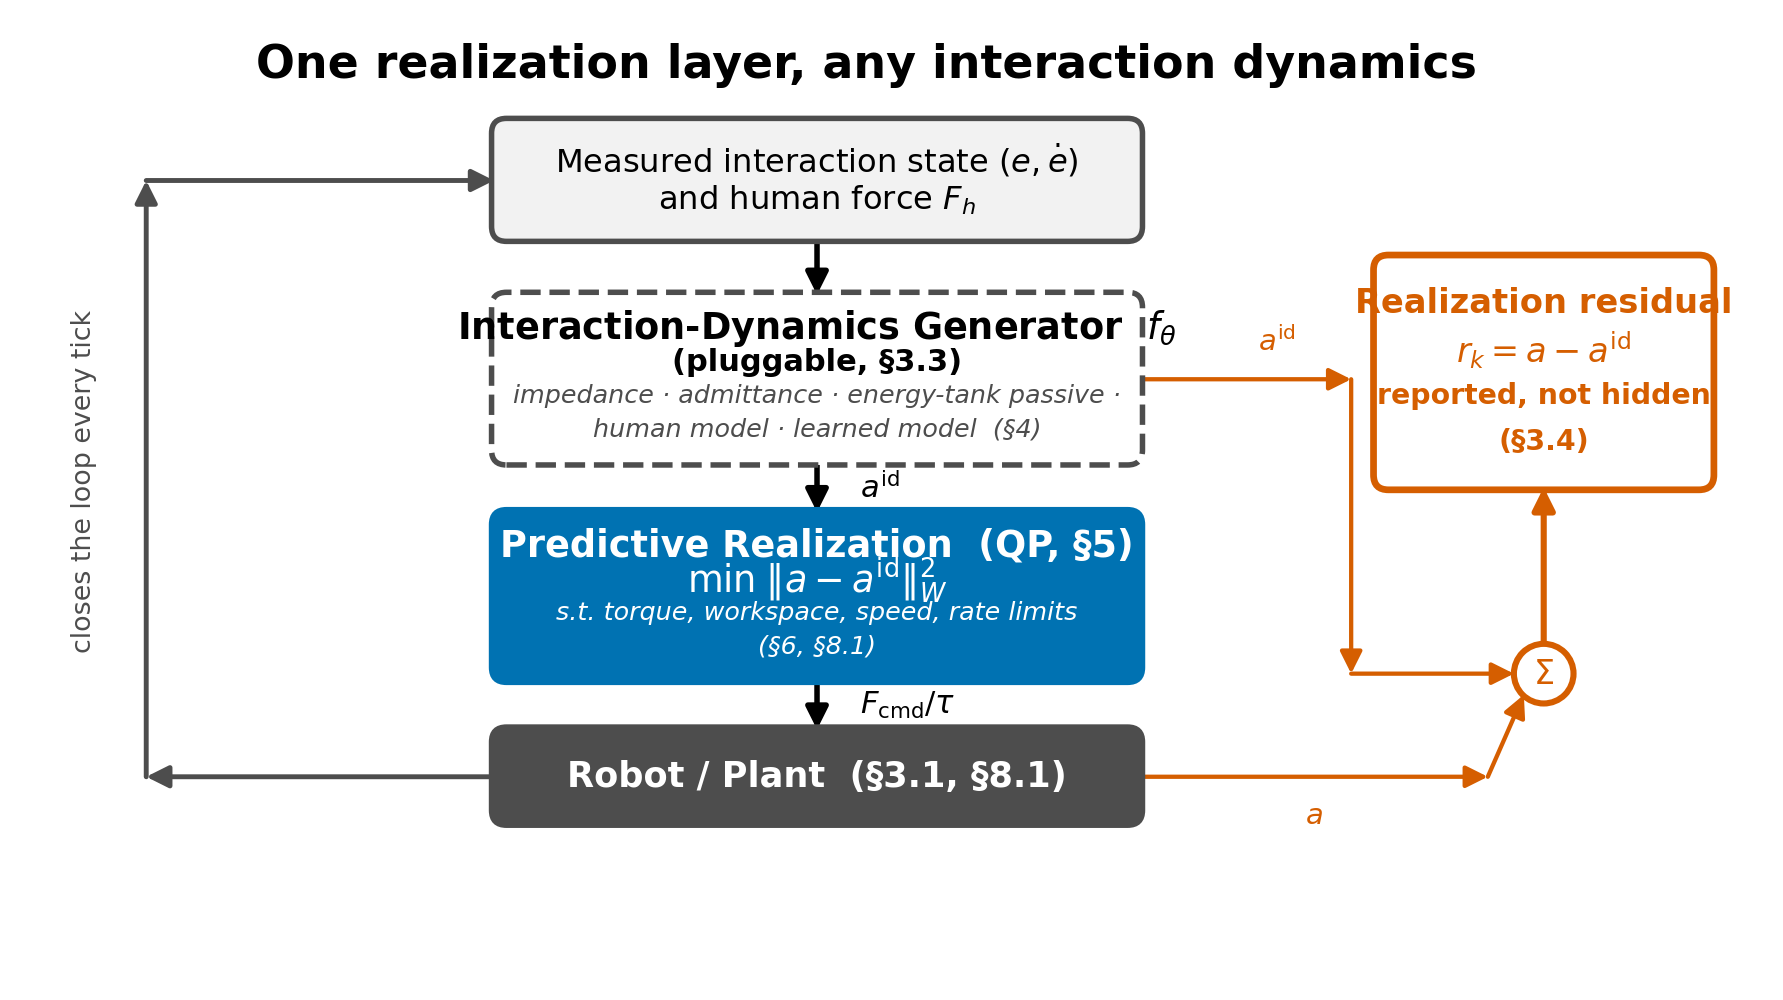
\includegraphics[width=0.95\linewidth]{results/architecture_diagram.png}
\caption{行为与实现是两个独立的层。行为层（虚线）提供 $a^{\mathrm{id}}$；实现运行时（蓝色）把它转换为一个受约束的指令，并报告 $r_k=a-a^{\mathrm{id}}$；式\eqref{eq:residual-decomposition}中的审计把它的成因分离开来。}
\label{fig:architecture}
\end{figure}

行为层表达意图，但不选择机器人指令。实现运行时负责可行性、约束强制执行与指令优化，而不决定刚度、阻尼或力响应语义应当意味着什么。运行时报告的是总行为误差与一个约束介入诊断量，而不是把二者混为一谈。

\noindent\textbf{当前的可执行实例。} 对于无记忆仿射行为模型，预测式运行时保持同一个决策变量、可行集与目标函数模板；期望的行为加速度通过 $(C_\theta,G_\theta)$ 进入。第~\ref{sec:properties}节形式化地给出了这一有限的结构性质，第~\ref{sec:generators}节实现了阻抗与导纳。非线性或有状态的说明可能需要不同的预测机制，按定义并不属于当前 QP 的实例。

这种分离改变了科学问题本身。我们不再问某个特定的 MPC 方案是否能产生柔顺的跟踪效果，而是问：

\begin{quote}
\emph{机器人控制软件应当如何把期望的交互行为，与其受约束的物理实现分离开来，又应当如何暴露不可避免的介入？}
\end{quote}

本文的贡献是：
\begin{itemize}
\item 一种行为--实现架构，把行为语义与物理指令可行性分配给不同的软件层；
\item 一个精确的期望加速度接口、一个总实现残差，以及一个同目标的受约束/无约束审计，使约束介入可以被单独观测到；
\item 一个针对无记忆仿射子类的预测式实现运行时，在阻抗与导纳两种行为层之间共享固定的机器人指令变量与可行集；
\item 可复现的平面与 FR3 仿真，展示了在线行为层替换、预见式状态约束处理，以及在指令与力矩限制下的机械臂级实现。
\end{itemize}

我们\textbf{并不}主张抽象意义上的架构分离、MPC 中的阻抗行为，或受约束的交互控制本身是新的。任务空间逆动力学、全身 QP、参考调节器与分层机器人控制器，早已把相关职责分离开来，而模型预测式阻抗与交互控制器也提供了重要的一体化方案。本文更狭窄的贡献，是以下四点的组合：(i) 一个沿预测状态求值、并以加速度层面的契约进行交换的交互律；(ii) 一套在各生成器之间保持固定的机器人指令运行时；(iii) 一个把实现残差分解开的同目标受约束/无约束反事实方案；以及 (iv) 无需重建运行时状态即可进行的在线生成器替换。可执行的证据覆盖了两种仿射行为。

\section{相关工作与定位}
\label{sec:related}

要区分最接近的文献，最好看预测层或自适应层优化的是什么量，以及机器人层控制器被要求复现的是什么量。

\begin{table*}[t]
\centering
\caption{与相关工作的定位对比}
\label{tab:related}
\small
\begin{tabular}{@{}>{\raggedright\arraybackslash}p{0.19\linewidth}
>{\raggedright\arraybackslash}p{0.27\linewidth}
>{\raggedright\arraybackslash}p{0.24\linewidth}
>{\raggedright\arraybackslash}p{0.16\linewidth}@{}}
\toprule
类别 & 行为表示方式 & 被优化的机器人层变量 & 预测所扮演的角色 \\
\midrule
预测式变阻抗 & $M_d,D_d,K_d$，常伴一条轨迹 & 阻抗参数和/或轨迹 & 选择柔顺行为 \\
参考模型自适应阻抗 & $M_d\ddot e+D_d\dot e+K_de=F_h$ & 自适应反馈参数 & 通常不涉及 \\
直接机器人 MPC & 状态或跟踪误差动力学 & 力、力矩、速度或加速度 & 直接优化机器人运动 \\
阻抗/交互 MPC & 阻抗、力，或耦合的交互模型 & 机器人指令，有时也含行为参数 & 把交互目标与约束嵌入优化问题 \\
参考调节器 & 单一的参考/设定点信号 & 送入固定内环控制器的经滤波参考 & 监督一个非预测式内环以满足约束 \\
预测安全滤波器 & 名义控制器输入 & 经最小修改的可行输入 & 认证或替换一个被提出的指令 \\
受约束柔顺性 QP & 期望阻抗/柔顺响应 & 力、速度或加速度 & 在机器人约束下复现柔顺行为 \\
TSID / 分层全身 QP & 期望任务加速度与任务优先级 & 关节加速度、接触力和/或力矩 & 通常是瞬时的受约束实现 \\
预测式分层任务空间控制 & 任务轨迹与加速度层面的误差 & 机器人状态与指令轨迹 & 把分层任务目标扩展到一个时域上 \\
本文 & $a^{\mathrm{id}}=C_\theta x+G_\theta F_h$ & 机器人指令 $u$ & 在约束下最小化动力学实现误差 \\
\bottomrule
\end{tabular}
\end{table*}

有若干方法用 MPC 来自适应地调整阻抗参数，或联合规划阻抗与运动。Anand 等人在一个底层变阻抗控制器之上放置了一个学习到的预测策略~\cite{ref1}。Haninger 等人预测交互，在线优化轨迹与阻抗，同时纳入安全约束~\cite{ref2}。近期的预测式变阻抗方案延续了这一参数自适应的方向~\cite{ref3}。它们所优化的行为变量是刚度、阻尼，或相关的轨迹参数。

一条相关的工作线是模型参考自适应阻抗控制，它说明期望的阻抗动力学，并设计一个自适应非线性控制器使机器人逼近它~\cite{ref4}。这确立了"把期望模型与物理机器人分离"这一做法的价值，但它本身并不提供对耦合状态与输入约束的全时域处理。

另一类方法把 MPC 直接应用于机器人本身或一个反馈线性化后的误差模型，其决策变量是机器人指令而不是阻抗参数。这样的控制器可以产生一个有效的闭环阻抗，但除非一个期望的交互模型显式地出现在预测目标中，否则这个阻抗只是优化器的一个诱导性质，而不是它被要求实现的那个行为。这一区分把本文的方案与我们此前的双积分器跟踪 MPC 区分开来：此前的控制器惩罚的是交互误差，而本文的控制器惩罚的是与一个独立说明的交互动力学系统之间的不一致。

任务空间逆动力学与分层全身 QP，是这一接口本身更基础的先例：它们早已把期望的任务加速度作为模块化目标接受下来，并求解出动力学可行的机器人加速度、接触力或力矩。以 Del Prete 等人的 TSID 为例，它处理的是受约束全驱动机器人的优先级化运动/力任务~\cite{ref19}。预测式分层任务空间控制把加速度误差目标扩展到一个有限时域上，用于欠驱动且受约束的机器人~\cite{ref20}。因此，"期望任务加速度"与"在机器人约束下的 QP 实现"都不是本文所主张的新东西。相对于这些框架，本文在此检验的贡献更窄：任务是一个沿预测状态求值的交互动力学律；同一套运行时在阻抗与导纳生成器之间被保留下来；其残差用一个同目标反事实方案被拆分开来；而生成器可以在线替换，无需重建运行时状态。

更接近的是模型预测式阻抗与交互控制。Bednarczyk 等人通过 MPC 表述阻抗行为，并处理速度、能量、加加速度等实际约束~\cite{ref5}。Gold 等人在最优控制问题中使用机器人模型与交互模型，表述模型预测式交互控制，并通过代价与约束表达操作目标~\cite{ref6}。Minniti 等人把全身 MPC 与机器人-环境交互模型的在线自适应结合起来，用于受约束的移动操作~\cite{ref7}。这些论文都是很接近的先例，使得"首个受约束交互动力学 MPC"这样宽泛的主张站不住脚。Alharbat 等人明确对比了 NMPC 阻抗、级联导纳与混合位置/力三种范式~\cite{ref14}；他们后来的预测式导纳控制器同时预测机器人状态与期望阻抗状态，遵守执行器约束，并在真实的空中物理交互中得到了验证~\cite{ref15}。Kumbhar 等人把导纳生成的方案传给 Digit 硬件上一个受约束的全身 QP~\cite{ref17}。这些都是比本文这项纯仿真研究更强的验证先例；本文所寻求的剩余区别，是跨行为固定不变的期望加速度契约本身，而不是预测式柔顺性这件事本身。

对柔顺行为进行 QP 实现，以及报告残差，这两点也早于本文的工作。Leboutet 等人在运动学与动力学约束下计算机器人指令，并在肢体无法实现所请求的柔顺性时传播广义力残差~\cite{ref16}。更近期的安全关键自适应阻抗工作，把一个名义阻抗律通过一个带关节状态与力矩约束的 QP 滤波，并给出了形式化的不变性与有界性结果~\cite{ref18}。因此，"QP 约束下的柔顺性"与"一个显式残差"，本文都不单独主张是新颖的。

参考调节器与预测安全滤波器，是与本文这种分离在架构上最接近的亲缘方法，来自与上文所述参数自适应和直接 MPC 工作不同的另一支文献。一个参考调节器位于一个固定的、已设计好的内环控制器上游，修改参考信号，使得由此产生的闭环轨迹满足约束~\cite{ref8}。这个类比是直接的：一个参考调节器同样把"被指令的东西"与"可以安全执行的东西"分离开来。区别在于预测发生在哪里，以及交换的是什么对象。一个参考调节器通常监督一个固定的内环，操纵的是一个参考信号；而本文的实现层本身就是预测式的，被交换的对象是一个沿预测交互状态求值的仿射期望加速度律。实现残差还额外度量了被请求的动力学与被交付的动力学之间的差距。预测安全滤波器同样接受一个任意的上游指令，并使用基于模型的备用优化来认证或修改它~\cite{ref13}。这一联系限制了新颖性的主张：贡献并不在于抽象意义上的分离，而在于它在交互动力学层面的表述与度量方式。

控制屏障函数（CBF）二次规划是另一种相关的架构模式，来自另一支文献：一个 CBF-QP 在每个节拍接受一个名义控制输入，并将其投影到由安全约束所定义的最小偏差可行集上~\cite{ref10}。本文的实现层在结构上与之相似——把一个被请求的行为以最小偏差投影到一个机器人可行集上——但被投影的对象是一个在滚动时域上求值的完整行为律，而不是单个名义输入。本文报告的是总偏差，且受约束/无约束反事实方案识别出的是其中的约束介入分量，而不是把每一个非零残差都当作安全动作。本文并未与一个 CBF-QP 滤波器或一个参考调节器实例做直接对比；第~\ref{sec:scope}节把与最接近的替代架构进行匹配对比列为待完成的工作。

定理~\ref{thm:invariance}是关于一个参数化二次规划的结构性陈述：对于仿射生成器类而言，QP 的决策变量、可行集与约束结构是固定的，只有其代价系数随生成器参数 $\theta$ 变化。这正是显式 MPC / 多参数 QP 文献所研究的对象~\cite{ref11,ref12}，它们把解映射 $\theta\mapsto U_k^\star(\theta)$ 刻画为分段仿射的。本文并未使用那套机制——QP 是在每个节拍在线求解的，而不是离线预先计算的——但定理~\ref{thm:invariance}最好被理解为把这一已确立的参数化 QP 结构应用到行为--实现接口上的一个实例，而不是关于二次规划的一个新的结构性事实。

上表中的大多数方法优化的是与某一种具体行为表示绑定的量：阻抗参数、自适应阻抗增益，或相对某个具体交互模型的机器人层跟踪。参考调节器与安全滤波器这两行在架构上最为接近。本文更狭窄的区别，在于一个交互层面的行为契约，其期望加速度与机器人可行性相互独立，再加上一个总残差与反事实介入审计。可执行与理论上的证据，仅限于无记忆仿射阻抗与导纳行为。

\section{行为--实现表述}
\label{sec:behaviors}

\subsection{行为--实现接口}
\label{sec:interface}

考虑一个刚性机械臂
\begin{equation}
M(q)\ddot q+C(q,\dot q)\dot q+g(q) =\tau+J(q)^\top F_h,
\end{equation}
其中 $q\in\mathbb R^{n_q}$，$\tau\in\mathbb R^{n_q}$，$F_h$ 是施加在交互端口上的人类力旋量。对于一个任务坐标
$y=h(q)\in\mathbb R^{n_y}$，
\begin{equation}
\dot y=J(q)\dot q, \qquad \ddot y=J(q)\ddot q+\dot J(q,\dot q)\dot q.
\end{equation}
代入关节动力学，得到仿射的加速度映射
\begin{equation}
\ddot y =b_y(q,\dot q,F_h)+G_y(q)\tau,
\end{equation}
其中
\begin{align}
b_y(q,\dot q,F_h) &= J M^{-1}\left(-C\dot q-g+J^\top F_h\right)+\dot J\dot q,\\
G_y(q)&=JM^{-1}.
\end{align}
令 $y_d$ 为一个名义交互位姿，定义
\begin{equation}
e=y-y_d, \qquad \dot e=\dot y-\dot y_d.
\end{equation}

\begin{definition}[行为层接口]
\label{def:interface}
在本架构中，行为层是一个因果映射
\begin{equation}
\ddot e^{\mathrm{id}} =f_\theta(e,\dot e,F_h,z),
\end{equation}
其中 $z$ 表示可选的内部行为状态，$\theta$ 表示行为参数。它的输出是一个期望的接触端口加速度——本文通篇称为\emph{期望行为加速度}——而不是一个机器人指令。行为层刻意不了解机器人力矩限制、关节限位或工作空间几何；这些属于实现层。这个一般性的映射定义了接口的边界；下文的定理与实验只覆盖它的无记忆仿射特化形式。
\end{definition}

本架构并不要求行为层计算 $\tau$。它提供 $\ddot e^{\mathrm{id}}$，由实现层选择 $\tau$，使物理的 $\ddot e$ 逼近 $\ddot e^{\mathrm{id}}$，同时满足机器人约束。下文给出的预测式 QP 是实现层的一种实现方式，而不是该层本身的定义。

完整的机械臂表述是目标架构。下面的平面研究使用如下精确离散化的特化形式，从而可以在没有运动学或逆动力学混杂因素的情况下，单独考察行为--实现分离：一个平面质点，
\begin{equation}
m_r\ddot p(t)=u(t)+F_h(t),
\end{equation}
其中 $p\in\mathbb R^2$ 是相对名义交互位姿的位移，$u\in\mathbb R^2$ 是被指令的机器人力，$F_h\in\mathbb R^2$ 是测得的人类力，$m_r>0$ 是被实现的机器人质量。定义
\begin{equation}
x=\begin{bmatrix}p^\top&v^\top\end{bmatrix}^\top,\qquad v=\dot p.
\end{equation}
在周期为 $\Delta t$ 的零阶保持下，
\begin{equation}
x_{k+1}=Ax_k+B(u_k+F_{h,k}),
\end{equation}
\begin{equation}
A= \begin{bmatrix} I&\Delta tI\\0&I \end{bmatrix}, \qquad
B= \begin{bmatrix} \frac{\Delta t^2}{2m_r}I\\ \frac{\Delta t}{m_r}I \end{bmatrix}.
\end{equation}
实际加速度为
\begin{equation}
a_k=\frac{u_k+F_{h,k}}{m_r}.
\end{equation}

对于这一平面被控对象，定义~\ref{def:interface}用 $x_k=[p_k^\top\ v_k^\top]^\top$ 特化替代了 $(e,\dot e)$：
\begin{equation}
a_k^{\mathrm{id}} =f_\theta(x_k,F_{h,k},z_k).
\end{equation}
对于本文通篇考虑的仿射类，
\begin{equation}
a_k^{\mathrm{id}}=C_\theta x_k+G_\theta F_{h,k}.
\end{equation}

一个行为所说明的量、与机器人实际交付的量之间的差距，就是\emph{总实现残差}，
\begin{equation}
r_k=a_k-a_k^{\mathrm{id}}.
\end{equation}
若 $r_k=0$，机器人在该采样点精确实现了期望行为加速度。然而，单独的非零 $r_k$ 并不能证明该偏差是由某个约束造成的：有限的力权重与力变化率权重本身就已经可以移动无约束最优解，而一个物理被控对象也可能与预测模型存在差异。

因此我们审计三个项。令 $U_k^{c\star}$ 为部署的受约束最优解，$U_k^{0\star}$ 为在同一状态、同一力预报与同一上一步指令下，去掉物理约束后、同一时域目标函数的反事实最优解。令 $a_k^c$ 与 $a_k^0$ 分别为它们的第一步模型加速度，令 $a_k^{\rm emp}$ 为从被控对象测得的加速度。定义
\begin{align}
r_k^{\rm reg}&=a_k^0-a_k^{\rm id}, &
r_k^{\rm con}&=a_k^c-a_k^0,\\
r_k^{\rm mod}&=a_k^{\rm emp}-a_k^c. &&
\end{align}
于是实测的总误差可精确闭合为
\begin{equation}
r_k^{\rm emp}=r_k^{\rm reg}+r_k^{\rm con}+r_k^{\rm mod}.
\label{eq:residual-decomposition}
\end{equation}
其中 $r^{\rm reg}$ 包含次级目标的折衷，$r^{\rm con}$ 是全部被强制执行的约束共同的介入量，$r^{\rm mod}$ 包含冻结模型误差与加速度测量误差。该分解并不把 $r^{\rm con}$ 归因于某一条具体被激活的约束行；那需要一个基于乘子或逐约束剔除的分析。对于精确的平面模型，$r^{\rm mod}=0$。FR3 审计在 50~Hz 的 manager 更新时刻求值前两项，并从随后 1~kHz 的被控对象采样中得到 $r^{\rm mod}$。

这四个量都保留物理加速度单位。它们是用于记录与因果诊断的信号，而不是跨生成器归一化的评分；一个按生成器归一化或按能量归一化的度量会回答一个不同的对比问题。

这一定义刻意比"指令一个名义阻抗力并惩罚
\begin{equation}
\left\|u_k-u_k^{\mathrm{imp}}\right\|_2^2
\end{equation}
"更强。后者是控制器输出层面的跟踪：它惩罚的是与一个名义力指令之间的偏差。$\|r_k\|_W^2$ 也是一种跟踪，但跟踪的是一个范畴上不同的目标——生成器所说明的\emph{期望行为加速度}，而不是某个先前控制器的输出——因此它是直接比较两个物理加速度。本文针对阻抗与导纳论证了这一区分，二者都不需要 QP 去跟踪某个先前控制器的输出。

\subsection{已实现的行为层}
\label{sec:generators}

下面实现的两个行为层，使用第~\ref{sec:qp}节所开发的同一个 QP 模板，仅在 $(C_\theta,G_\theta)$ 上有所不同，如定理~\ref{thm:invariance}所形式化的那样。第一个是阻抗生成器，其期望阻抗为
\begin{equation}
M_d a^{\mathrm{id}}+D_dv+K_dp=F_h.
\end{equation}
对各向同性参数，
\begin{equation}
a^{\mathrm{id}} =-\frac{K_d}{M_d}p-\frac{D_d}{M_d}v+\frac{1}{M_d}F_h,
\end{equation}
因此
\begin{equation}
C_{\mathrm{imp}} =\begin{bmatrix} -K_dM_d^{-1}I&-D_dM_d^{-1}I \end{bmatrix},
\qquad G_{\mathrm{imp}}=M_d^{-1}I.
\end{equation}
与变阻抗 MPC（第~\ref{sec:related}节）不同，本表述中 $M_d,D_d,K_d$ 不是决策变量；它们描述的是被请求的行为。

第二个是力引导的导纳生成器，它请求一个与力相关的速度：
\begin{equation}
T_a a^{\mathrm{id}}+v=YF_h,
\end{equation}
即
\begin{equation}
a^{\mathrm{id}}=-T_a^{-1}v+T_a^{-1}YF_h.
\end{equation}
它没有位置恢复项。力释放之后，速度衰减，但已产生的位移会被保留。它通过同一个加速度接口，提供了一种性质截然不同的行为。

\subsection{预测式实现运行时}
\label{sec:qp}

第~\ref{sec:generators}节给出 $a^{\mathrm{id}}$。对一个无记忆仿射生成器而言，它由 $C_\theta,G_\theta$ 表示，产生一个统一的浓缩 QP 模板，其数值代价系数随生成器变化，而其决策变量与可行集不变。在时刻 $k$，令
\begin{equation}
U_k= \begin{bmatrix} u_{0|k}^\top&\cdots&u_{N-1|k}^\top \end{bmatrix}^\top.
\end{equation}
控制器求解
\begin{equation}
\begin{aligned}
\min_{U_k}\quad& \sum_{i=0}^{N-1}\Big(
\|a_{i|k}-a_{i|k}^{\mathrm{id}}\|_W^2
+\lambda_u\|u_{i|k}\|_2^2\\
&\hspace{25mm}+\lambda_{\Delta u}
\|u_{i|k}-u_{i-1|k}\|_2^2\Big)\\
\text{s.t.}\quad&x_{i+1|k}=Ax_{i|k}+B(u_{i|k}+\hat F_{h,i|k}),\\
&a_{i|k}=(u_{i|k}+\hat F_{h,i|k})/m_r,\\
&a_{i|k}^{\mathrm{id}} =C_\theta x_{i|k}+G_\theta\hat F_{h,i|k},\\
&|u_{i|k}|_\infty\le u_{\max},\\
&|u_{i|k}-u_{i-1|k}|_\infty \le\dot u_{\max}\Delta t,\\
&|p_{i+1|k}|_\infty\le p_{\max},\\
&|v_{i+1|k}|_\infty\le v_{\max}.
\end{aligned}
\end{equation}
只有 $u_{0|k}^\star$ 被执行。在 $i=0$ 的速率惩罚项与速率约束中出现的 $u_{-1|k}$，指的是上一次求解时实际施加的指令，由控制器在两次调用之间携带（在第一次求解之前为零），因此从第一次调用起二者就都是良定义的。实现中使用的是把测得的力在整个时域上保持不变，$\hat F_{h,i|k}=F_{h,k}$，而不是对脚本化力的先知式了解。可以在不改变生成器接口的情况下，替换为一个学习到的或基于物理的力预测器。

目标函数 $\|a_{i|k}-a_{i|k}^{\mathrm{id}}\|_W^2$ 是一种跟踪——但跟踪的是一个与位置或速度轨迹范畴上不同的目标。没有构造任何期望位置轨迹；优化器比较的是在预测交互状态下求值的两个加速度：受约束机器人将会产生的加速度，与生成器所说明的期望行为加速度。位置与速度作为生成器状态、以及作为受安全约束的量而出现，从不作为被跟踪的参考本身出现。

优化变量是机器人指令序列 $U_k$，而不是生成器的参数。生成器参数 $\theta$ 在每次实验中都是固定的。从阻抗切换到导纳，改变的是 $C_\theta,G_\theta$，而不是 QP 的约束或指令变量——这一点由定理~\ref{thm:invariance}（第~\ref{sec:properties}节）正式陈述。

\section{仿射运行时实例的性质}
\label{sec:properties}

本架构并不依赖下面这条 QP 性质；相反，这条性质展示的是，对于当前这个仿射子类而言，这种分离实现得有多干净。本节确立了模板不变性、凸性、理想条件下的精确实现，以及单步约束继承性，而命题~\ref{prop:inheritance}则明确陈述了运行时\emph{不}保证的东西。

\begin{theorem}[仿射生成器模板不变性性质]
\label{thm:invariance}
固定被控对象 $(A,B,m_r)$、时域长度 $N$、权重 $(W,\lambda_u,\lambda_{\Delta u})$，以及界 $(u_{\max},\dot u_{\max},p_{\max},v_{\max})$。存在唯一一个映射 $(C,G)\mapsto Q(C,G)$——一个只依赖于上述被控对象、时域、权重与界、而从不依赖于 $\theta$ 的二次规划模板——使得对每一个具有仿射律 $(C_\theta,G_\theta)$ 的生成器 $\theta$，第~\ref{sec:qp}节的实现 QP 恰好等于 $Q(C_\theta,G_\theta)$。因此，对任意两个生成器 $\theta_1,\theta_2$，实例 $Q(C_{\theta_1},G_{\theta_1})$ 与 $Q(C_{\theta_2},G_{\theta_2})$ 共享同一个决策变量 $U_k$ 与同一个可行集，二者的差异仅在于由 $(C_\theta,G_\theta)$ 贡献的数值目标系数，而不在于决策变量维数、约束集或目标函数模板。因此，实现一个不同的仿射生成器，改变的只是所提供的 $(C_\theta,G_\theta)$。一个非线性生成器会使 $a_{i|k}^{\mathrm{id}}$ 在 $U_k$ 中非线性，因此残差代价不再保证是凸二次的，模板 $Q$ 在不经线性化的情况下不适用。
\end{theorem}

\begin{proof}
第~\ref{sec:qp}节 QP 中的每一条约束——动力学递推式、加速度定义式，以及四个盒约束——都仅用 $A$、$B$、$m_r$、$u_{\max}$、$\dot u_{\max}$、$p_{\max}$、$v_{\max}$、$U_k$，以及由此产生的状态/加速度序列写出；没有一条引用 $\theta$、$C_\theta$ 或 $G_\theta$。因此可行集是一个固定的多面体，对每个生成器都相同。$(C_\theta,G_\theta)$ 在整个问题中唯一出现的地方，是主代价内的项 $a_{i|k}^{\mathrm{id}}=C_\theta x_{i|k}+G_\theta\hat F_{h,i|k}$，它在每个时域步中恰好出现一次，作为对 $r_{i|k}=a_{i|k}-a_{i|k}^{\mathrm{id}}$ 的一次仿射代入。由于 $x_{i|k}$ 本身与 $(C_\theta,G_\theta)$ 无关、且在 $U_k$ 中是仿射的（在下文命题~\ref{prop:convexity}的证明中确立），$a_{i|k}^{\mathrm{id}}$ 在 $U_k$ 中是仿射的，其系数仅依赖于 $(C_\theta,G_\theta)$，因此 $\|r_{i|k}\|_W^2$ 是 $U_k$ 中的一个凸二次型，其 Hessian 与梯度贡献完全由 $(C_\theta,G_\theta)$ 决定；次级项 $\lambda_u\|u_{i|k}\|_2^2$ 与 $\lambda_{\Delta u}\|u_{i|k}-u_{i-1|k}\|_2^2$ 则完全不涉及 $(C_\theta,G_\theta)$。把这些部分汇总起来，就把 $Q(C,G)$ 定义为一个仅依赖于 $(C,G)$ 的函数——被控对象、时域、权重与界作为固定参数进入 $Q$，而不是作为自变量——由构造可知，$Q(C_\theta,G_\theta)$ 恰好就是第~\ref{sec:qp}节针对生成器 $\theta$ 所给出的那个 QP。
\end{proof}

这正是为什么第~\ref{sec:generators}节中已实现的两个生成器是可核查的，而不只是一种设想：每一个都向同一个模板 $Q$ 提供一组不同的 $(C_\theta,G_\theta)$。在不经线性化的情况下，一个非线性或有状态的 $f_\theta$ 无法分解为一对固定的 $(C,G)$，因而不在该定理的适用范围内。

\begin{proposition}[仿射生成器下的凸性]
\label{prop:convexity}
若 $W\succeq0$、$\lambda_u\ge0$ 且 $\lambda_{\Delta u}\ge0$，则第~\ref{sec:qp}节中的有限时域问题是一个凸二次规划。若组装出的 Hessian 正定——包括常见情形 $\lambda_u>0$——则它是严格凸的。
\end{proposition}

\begin{proof}
由递推式 $x_{i+1|k}=Ax_{i|k}+B(u_{i|k}+\hat F_{h,i|k})$ 从 $x_{0|k}$ 展开可知，被提升的状态 $x_{i|k}$ 在 $U_k$ 中是仿射的。因此 $a_{i|k}=(u_{i|k}+\hat F_{h,i|k})/m_r$ 与 $a_{i|k}^{\mathrm{id}}=C_\theta x_{i|k}+G_\theta\hat F_{h,i|k}$ 在 $U_k$ 中都是仿射的，从而 $r_{i|k}=a_{i|k}-a_{i|k}^{\mathrm{id}}$ 在 $U_k$ 中是仿射的，且由于 $W\succeq0$，$\|r_{i|k}\|_W^2$ 是凸二次的。正则化项 $\lambda_u\|u_{i|k}\|_2^2$ 与 $\lambda_{\Delta u}\|u_{i|k}-u_{i-1|k}\|_2^2$ 在 $\lambda_u,\lambda_{\Delta u}\ge0$ 时，在 $U_k$ 中都是凸二次的，凸函数之和仍是凸的。所列出的每一条约束，都对 $U_k$ 的一个仿射函数取绝对值加以约束，因此可行集是若干半空间的交集，从而是一个凸多面体。
\end{proof}

\begin{proposition}[无约束下的精确实现]
\label{prop:exact}
另外假设 $W\succ0$（严格正定——比命题~\ref{prop:convexity}的 $W\succeq0$ 更强的假设）。假设存在一个输入序列，使得在整个时域上 $r_{i|k}=0$ 且没有任何约束被激活。若实现残差在次级努力目标之前按字典序被优先优化——或者等价地，次级权重为零——那么每一个最优的主目标解都精确实现了参考动力学。
\end{proposition}

\begin{proof}
主目标 $\sum_i\|r_{i|k}\|_W^2$ 非负，且在假设的可行序列处取值为零，因此它在整个时域上的最小值为零。在字典序优先（或次级权重为零）的条件下，任意最优解都必须达到这一最小值，因此 $\sum_i\|r_{i|k}\|_W^2=0$，又因为每一项都非负，所以对每个 $i$ 都有 $\|r_{i|k}\|_W^2=0$。由于 $W\succ0$，一个二次型 $\|r\|_W^2$ 只在 $r=0$ 处为零；若 $W$ 只是半正定，这一步只能得到 $r_{i|k}\in\ker W$，而不是 $r_{i|k}=0$，这正是为何此处需要更强的假设，而命题~\ref{prop:convexity}中则不需要。
\end{proof}

在次级权重有限（而非为零）的情况下，即便在无约束的时段内，预测式实现所测得的残差也不精确为零（表~\ref{tab:planar}），这与命题~\ref{prop:exact}的零权重理想化情形是一致的。反应式对比方案求解的则是生成器瞬时律的一个不同的、无约束的代数求逆，因此其残差处于数值求解器容差水平（表~\ref{tab:planar}）——这只是一次对底层生成器与动力学模型实现是否正确的检验，本身并不是命题~\ref{prop:exact}的一个实例。

\begin{proposition}[单步约束继承性]
\label{prop:inheritance}
假设模型与当前人类力在被执行的采样点上是精确的，且 QP 可行。那么 $u_{0|k}^\star$、$p_{1|k}$ 与 $v_{1|k}$ 满足各自对应的 QP 界。在每个采样点都重新求解，通过归纳可得到约束满足性，同时保持可行性。
\end{proposition}

这条命题不是一个递归可行性定理。一个可部署的版本，需要一个终端不变集、带有量化后备方案的软约束，或一个后备安全控制器。单个采样点内的突发力变化以及模型误差，也必须由鲁棒的约束收紧来覆盖。

\section{平面架构验证}
\label{sec:planar}

第~\ref{sec:properties}节确立了 QP 在原理上保证什么——凸性、无约束时的精确实现、单步约束满足——以及它不保证什么（递归可行性）。本节在第~\ref{sec:interface}节的平面被控对象上，从经验上检验这些性质，在相同的指令与速率限制下，把预测式实现与反应式对比方案进行比较。

\subsection{可复现设置}

仿真使用一个 2.5~kg 的平面质点，$\Delta t=0.02$~s，20 步（0.4~s）时域。沿 $+y$ 方向施加一个平滑的 12~N 力，从 1~s 持续到 3~s。限制为
\begin{equation}
|u_j|\le18\text{ N},\qquad |v_j|\le0.22\text{ m/s},\qquad
|p_j|\le0.10\text{ m},
\end{equation}
且 $|\dot u_j|\le180$~N/s。实现、力与力变化率的权重分别为 $1$、$2\times10^{-4}$ 与 $10^{-3}$。

阻抗生成器（第~\ref{sec:generators}节）使用
\begin{equation}
M_d=2.0\text{ kg},\quad D_d=18\text{ Ns/m},\quad K_d=45\text{ N/m}.
\end{equation}
导纳生成器（第~\ref{sec:generators}节）使用 $T_a=0.25$~s，$Y=0.025$~m/(Ns)。

对比方案计算瞬时参考加速度，将其转换为机器人力，并施加同样的 18~N 力与 180~N/s 速率限制。它不对位置或速度约束做任何预测。这个对比方案是刻意做到最小化的：它只用来隔离出全时域状态约束改变了什么；它并不被当作一个覆盖全面的基线。

\subsection{结果}
\label{sec:planar-results}

\begin{figure}[t]
\centering
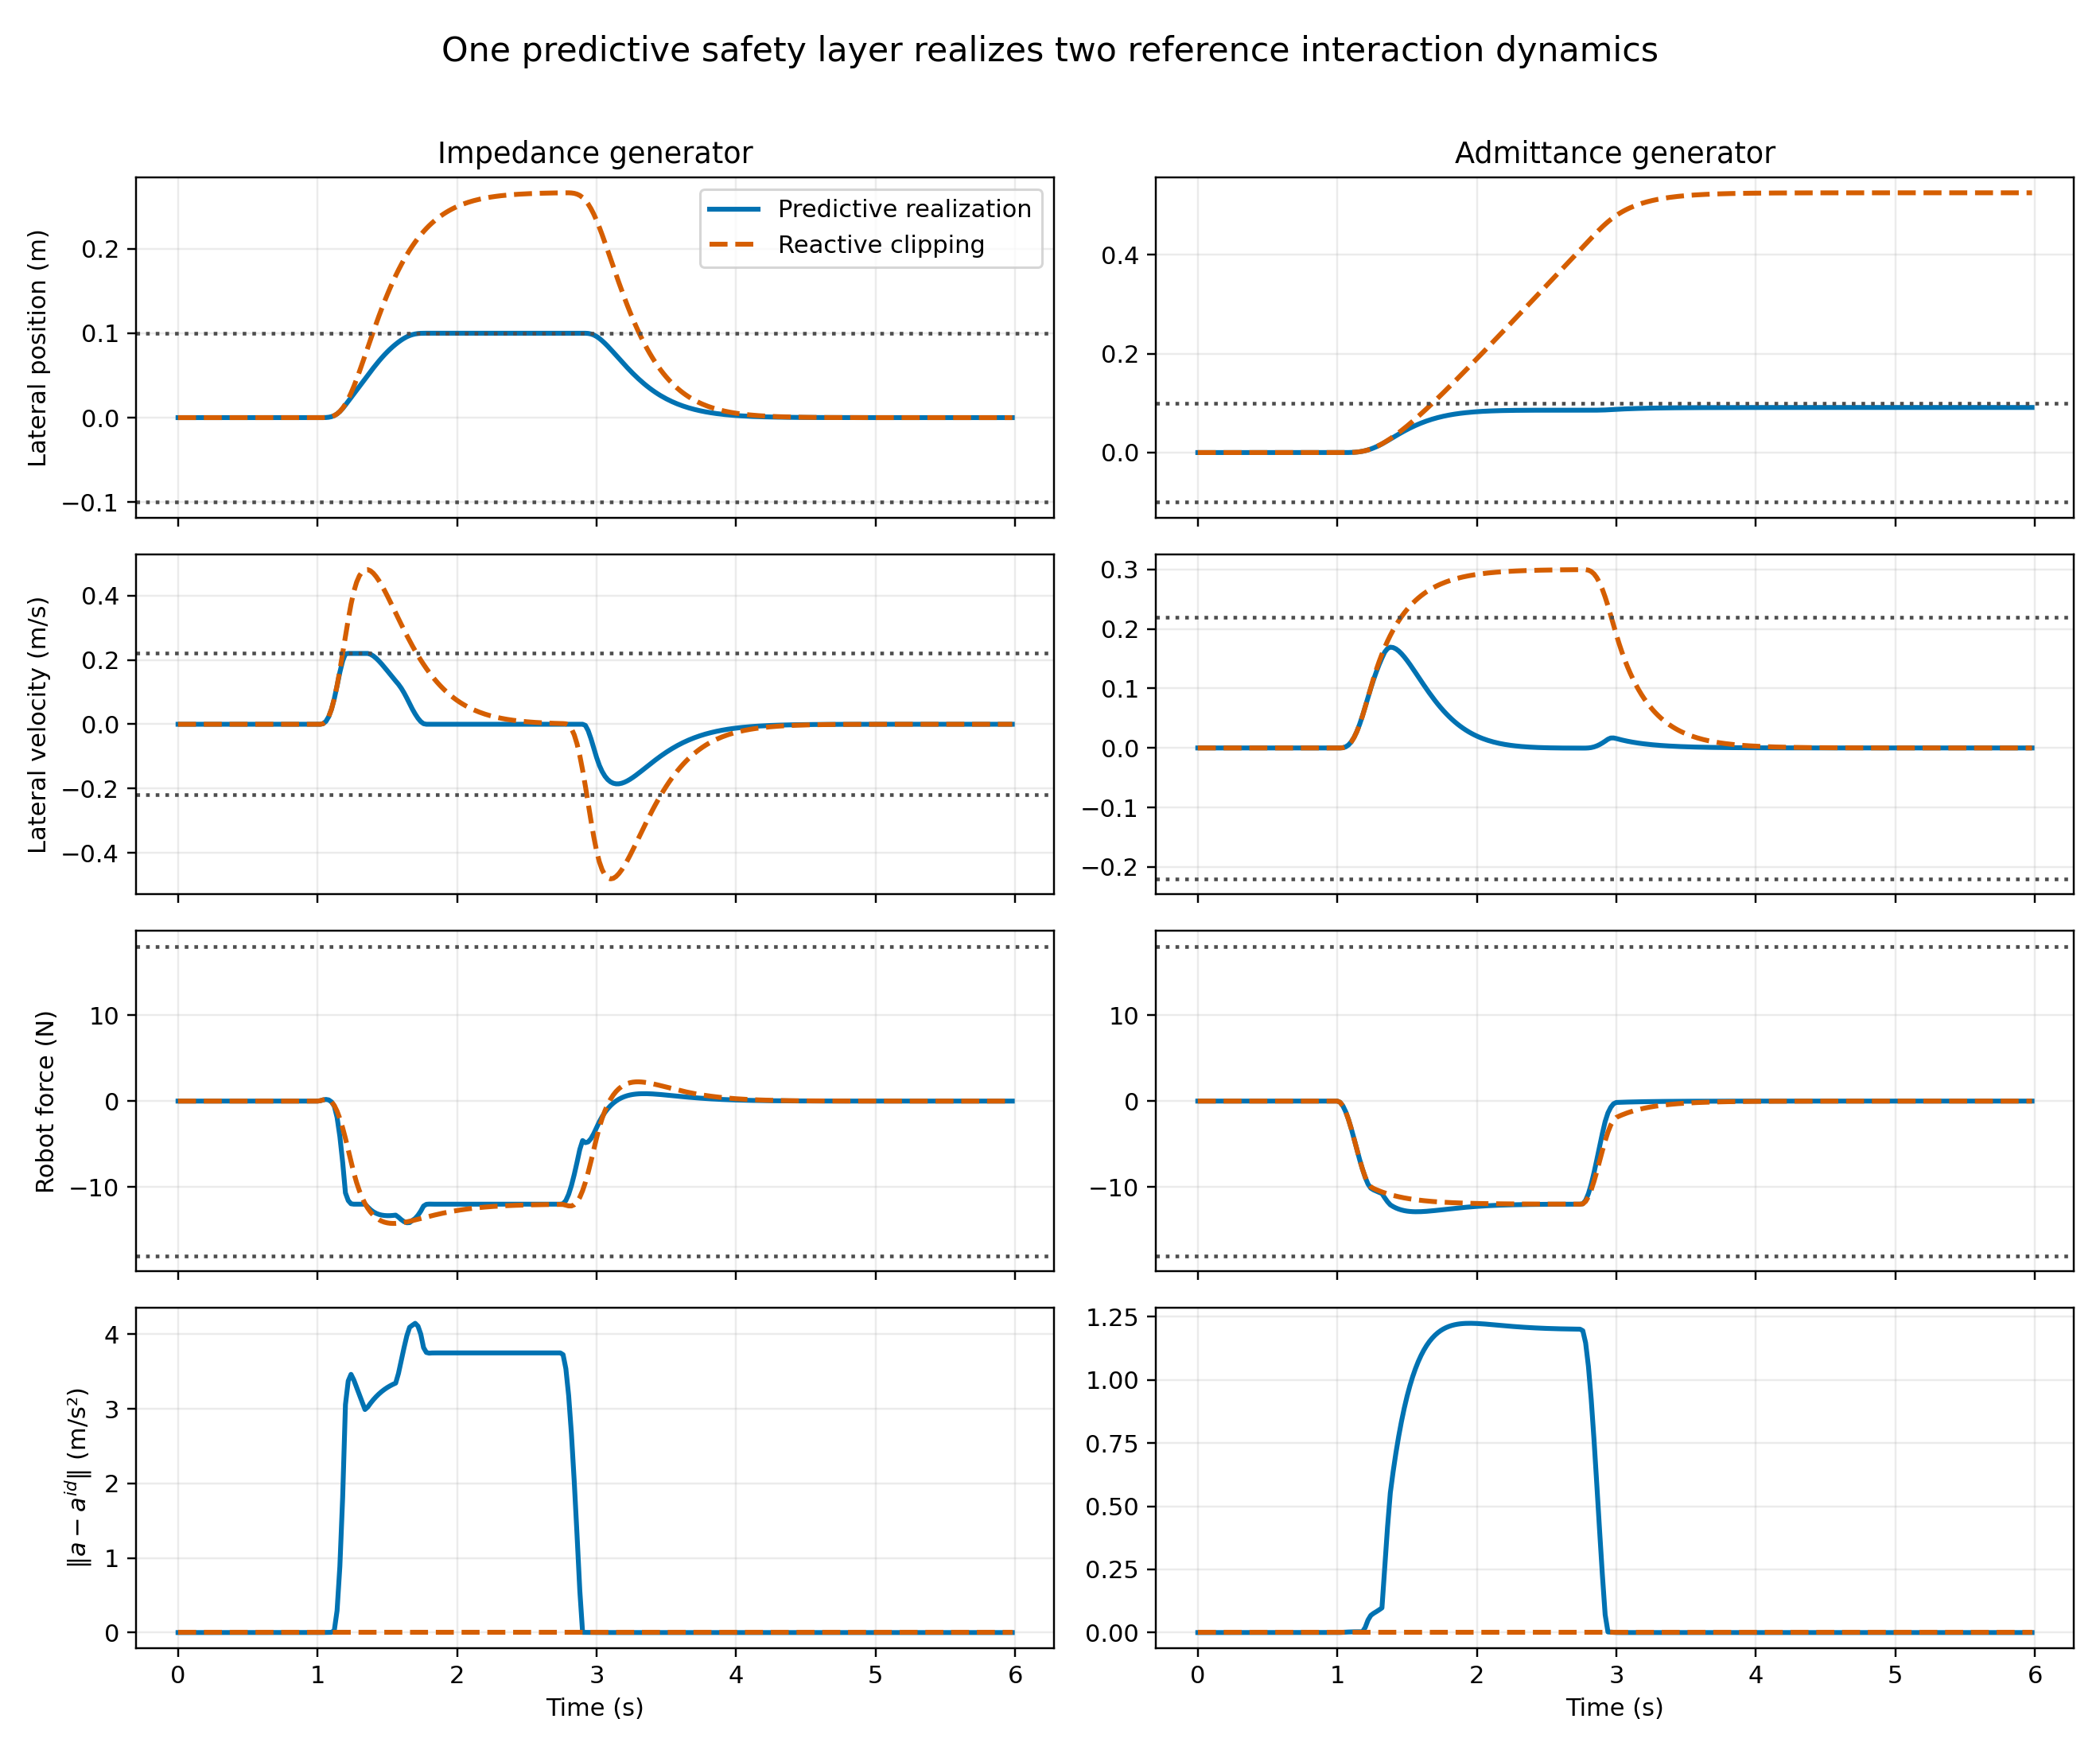
\includegraphics[width=0.95\linewidth]{results/interaction_dynamics_results.png}
\caption{平面验证：阻抗（左）与导纳（右）。虚线为状态限制。反应式截断跟踪行为但忽略限制；预测式实现在接近边界处偏离它（最后一行）。}
\label{fig:planar}
\end{figure}

\begin{table*}[t]
\centering
\caption{平面验证}
\label{tab:planar}
\small
\begin{tabular}{@{}llrrrrl@{}}
\toprule
生成器 & 控制器 & RMSE$^{*}$ & 峰值 $|p_j|$ & 峰值速度 & 峰值 $|u_j|$ & 违反量 \\
& & (m/s$^2$) & (m) & (m/s) & (N) & \\
\midrule
阻抗 & 预测式 & 1.351 & 0.100002 & 0.220 & 14.16 & $2\times10^{-6}$~m \\
阻抗 & 反应式 & $<10^{-6}$ & 0.2663 & 0.480 & 14.24 & 0.1663~m, 0.260~m/s \\
导纳 & 预测式 & 0.405 & 0.0912 & 0.169 & 12.88 & 无 \\
导纳 & 反应式 & $<10^{-6}$ & 0.5250 & 0.300 & 12.00 & 0.4250~m, 0.080~m/s \\
\bottomrule
\end{tabular}

\vspace{2pt}
\raggedright\footnotesize
$^{*}$实现 RMSE，按分量计算。状态限位违反量报告的是超出 0.10~m / 0.22~m/s 工作空间/速度界的量。反应式对比方案的实现 RMSE 处于数值求解器容差水平，因为它直接对生成器的瞬时律求逆；预测式实现非零的残差，反映的是有限的次级权重与约束驱动的偏差，在整次运行中累积（命题~\ref{prop:exact}，第~\ref{sec:properties}节）。与表~\ref{tab:fr3}一样，RMSE 是\emph{按分量}计算的：所有残差分量与所有时间采样点先汇总为一个均值，再开方。
\end{table*}

\begin{table}[t]
\centering
\caption{平面残差分解（m/s$^2$）}
\label{tab:planar-decomposition}
\small
\begin{tabular}{@{}lrrrr@{}}
\toprule
生成器 & 总量 & $r^{\rm reg}$ & $r^{\rm con}$ & 闭合误差 \\
\midrule
阻抗  & 1.351 & 0.0113 & 1.339 & $<9\!\times\!10^{-16}$ \\
导纳 & 0.405 & 0.00261 & 0.403 & $<3\!\times\!10^{-16}$ \\
\bottomrule
\end{tabular}

\vspace{2pt}
\raggedright\footnotesize
前三个数值列是按分量计算的 RMSE，不需要作为标量相加；式\eqref{eq:residual-decomposition}是逐样本闭合的。"闭合误差"是其最大绝对分量误差。平面模型是精确的，因此 $r^{\rm mod}=0$。
\end{table}

阻抗参考的静态位移为 $F_h/K_d=12/45=0.267$~m，与平滑力斜坡之后实测的 0.266~m 峰值相符。由于这一行为与 0.10~m 的工作空间不相容，预测式控制器在边界被激活期间增大了实现残差。力释放之后，它回到位于原点的阻抗平衡点。

导纳参考在 12~N 下请求约 0.30~m/s 的速度，且没有恢复弹簧。因此反应式实现累积了 0.525~m 的位移，并在力释放之后仍保留该位移。受约束的控制器在到达工作空间边界之前就已开始偏离所请求的速度动力学，最终稳定在 0.091~m。生成器本身保持不变。表~\ref{tab:planar-decomposition}显示，观测到的修正主要是约束介入，而不是次级正则化；更强的"完全由约束引起"这种措辞会是错误的，因为正则化项虽小但非零。

\subsection{在线生成器切换}
\label{sec:switching}

前两小节通过分别运行两次仿真——每个生成器一次——验证了生成器接口，这很有信息量，但还不足以证明同一个运行中的控制器可以在不重新设计的情况下接受一个不同的生成器。本节直接检验这一点。构造一个 \texttt{InteractionDynamicsMPC} 实例，仅一次，使用阻抗生成器；在整个 6~s 运行期间施加一个很小的横向恒力（1~N，远在每一个界之内），不释放。在 $t=2$~s 与 $t=4$~s，在这个运行中的控制器上恰好重新指派一个属性——\texttt{controller.generator}——依次切换阻抗 $\rightarrow$ 导纳 $\rightarrow$ 阻抗；除此之外没有任何其他东西（QP 权重、约束、决策变量，或在两次求解之间携带的 \texttt{previous\_command} 状态）被触碰或重建。

\begin{figure}[t]
\centering
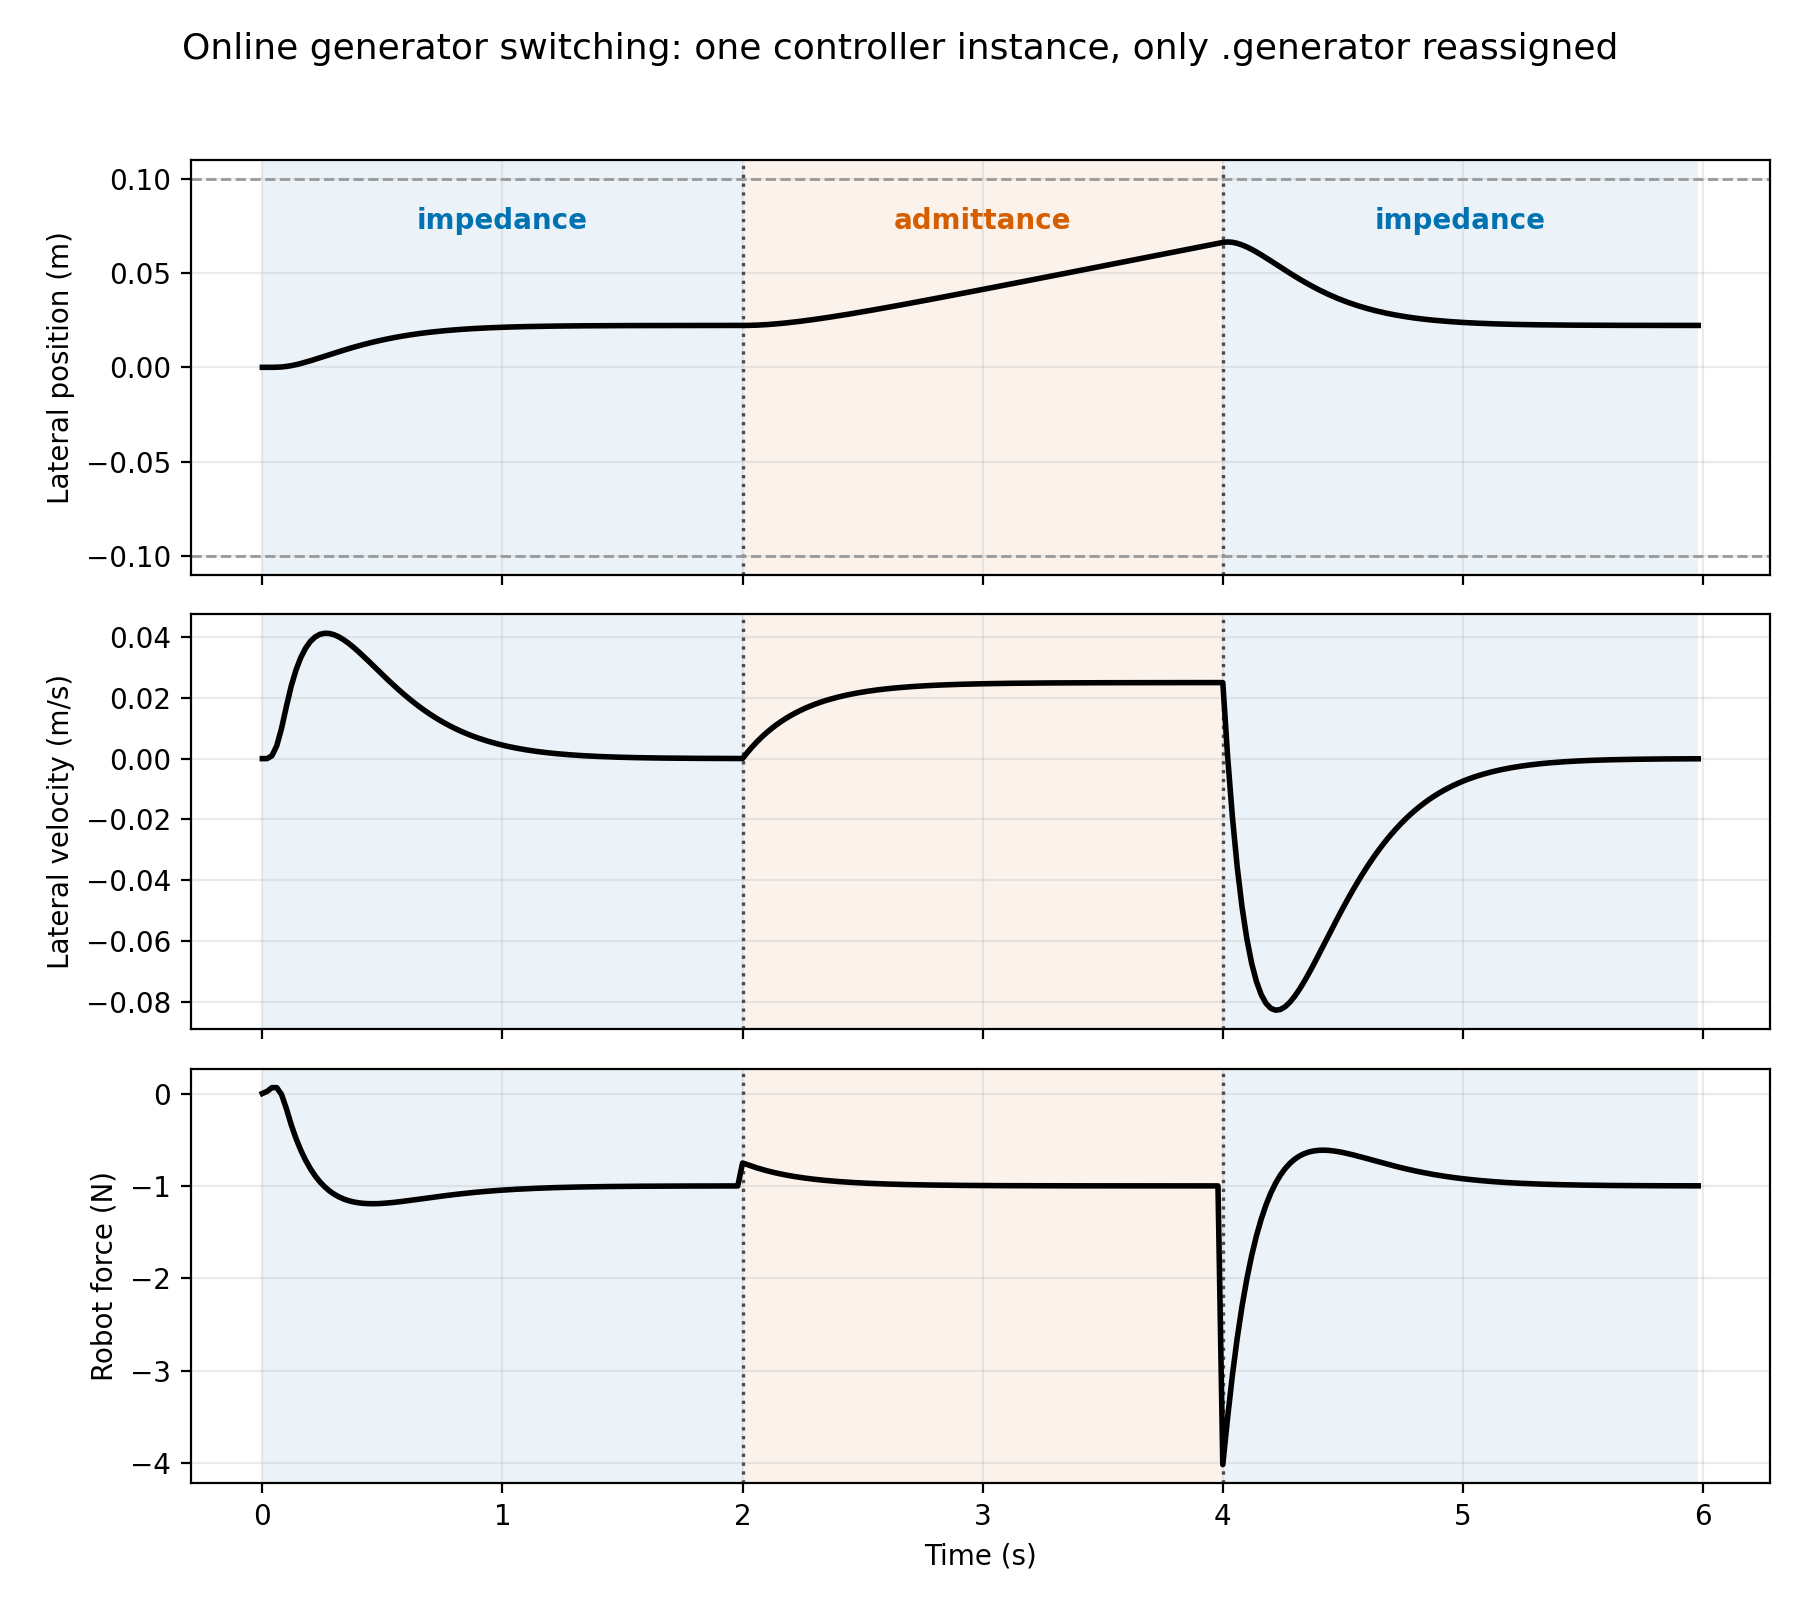
\includegraphics[width=0.9\linewidth]{results/generator_switching_results.png}
\caption{单个控制器实例；仅在 $t=2$~s 与 $t=4$~s 重新指派 \texttt{.generator}。位置在两段阻抗区间内都收敛到阻抗平衡点，在两者之间的导纳区间内漂移，并在从一个不同的状态重新进入后重新收敛。}
\label{fig:switching}
\end{figure}

两次切换都是受速率约束的：在切换时刻，最大的指令力跳变发生在 $t=4$~s，为 3.02~N，是 QP 每节拍 3.6~N 限制的 84\%。这是一次实质性的指令变化，而不是数学光滑性的证据；它只是满足了约束每一个其他步骤的同一个离散速率约束。位置与速度在整个过程中都始终保持在距原点 0.067~m 与 0.083~m 以内，远在 0.10~m / 0.22~m/s 的界之内。因此，该实验验证的是软件层面的生成器接口，以及在现有速率约束下在线切换的可行性；它并不确立最优切换、混合稳定性，或生成器律的连续性。第二段阻抗区间还额外展示了：从导纳区间遗留下来的、不同的位置与非零速度出发，无需针对重新进入做特殊处理，也能重新收敛。

\subsection{实验所确立的结论}

这些结果支持四条有限的主张：
\begin{enumerate}
\item 两种性质不同的仿射交互模型，使用同一套受约束的预测式实现；
\item 一个受约束/无约束反事实方案，把约束介入与总行为误差中较小的正则化分量区分开来；
\item 在这个确定性模型中，全时域状态约束能够防止仅靠指令截断无法防止的违反；
\item 单个运行中的控制器实例，可以在运行途中通过重新指派一个属性，在线接受一个不同的生成器，其指令变化被现有的速率约束所限定。
\end{enumerate}
它们并不确立机械臂层面的可行性、耦合的人机稳定性、无源性、对力估计延迟的鲁棒性，或在嵌入式硬件上的实时性能。

\section{FR3 运行时验证}
\label{sec:fr3}

第~\ref{sec:planar}节通过使用一个质点，把行为--实现分离与运动学、逆动力学等混杂因素隔离开来。本节把同一个接口部署在一台 MuJoCo 中力矩控制的 7 自由度 Franka FR3 上，用第~\ref{sec:interface}节非线性的、随构型变化的机械臂动力学，替换掉精确的双积分器被控对象。

\subsection{架构}
\label{sec:fr3-architecture}

在每次求解时，令 $J_v(q)\in\mathbb R^{3\times7}$ 为平移雅可比矩阵，$\Lambda(q)^{-1}=J_vM(q)^{-1}J_v^\top$ 为位置坐标所对应的（经正则化的）操作空间惯量的逆。

\noindent\textbf{完整闭环律。} 令 $R_d$ 为被保持的参考姿态，$e_R(q)\in\mathbb R^3$ 为相应的姿态误差，$J_w(q)\in\mathbb R^{3\times7}$ 为旋转雅可比矩阵，$q_0$ 为一个固定的中性构型。指令关节力矩由一个前馈项 $\tau_{\mathrm{ff}}$、一个原始姿态保持项 $\tau_{\mathrm{orient}}$、一个原始零空间定心项 $\tau_{\mathrm{null}}$，以及它们通过零空间投影算子 $\bar N_v$ 投影后得到的 $\tau_{\mathrm{aux}}$ 组装而成：
\begin{equation}
\begin{aligned}
\tau_{\mathrm{ff}}(q,\dot q)&=C(q,\dot q)\dot q+g(q),\\
\tau_{\mathrm{orient}}(q,\dot q)&=J_w(q)^\top\bigl(-K_{\mathrm{rot}}e_R(q)-D_{\mathrm{rot}}\omega\bigr),\\
\tau_{\mathrm{null}}(q,\dot q)&=-k_{\mathrm{null}}(q-q_0)-d_{\mathrm{null}}\dot q,\\
\bar N_v(q)&=I_7-M(q)^{-1}J_v(q)^\top\Lambda(q)\,J_v(q),\\
\tau_{\mathrm{aux}}(q,\dot q)&=\bar N_v(q)^\top\bigl[\tau_{\mathrm{orient}}(q,\dot q)+\tau_{\mathrm{null}}(q,\dot q)\bigr],\\
\tau_{\mathrm{base}}(q,\dot q)&=\tau_{\mathrm{ff}}(q,\dot q)+\tau_{\mathrm{aux}}(q,\dot q),
\end{aligned}
\end{equation}
被执行的力矩为
\begin{equation}
\tau=\tau_{\mathrm{base}}(q,\dot q)+J_v(q)^\top F_{\mathrm{cmd}}.
\end{equation}
任务加速度满足 $\ddot y=J_v\ddot q+\dot J_v\dot q$。因此，定义
\begin{equation}
d_{\mathrm{known}}(q,\dot q) =J_v(q)M(q)^{-1}\tau_{\mathrm{aux}}(q,\dot q)
+\dot J_v(q,\dot q)\dot q,
\end{equation}
它同时包含了被投影的辅助力矩贡献与任务运动学项。QP 所使用的残差平移动力学为
\begin{equation}
\ddot e=\Lambda(q)^{-1}\bigl(F_{\mathrm{cmd}}+F_h\bigr)+d_{\mathrm{known}},
\end{equation}
其中实现的加速度在被指令的力上是\emph{正}的，与第~\ref{sec:interface}节的质点约定一致。$F_{\mathrm{cmd}}\in\mathbb R^3$ 是 QP 的笛卡尔修正力，由当前被激活的控制器提供。预测式控制器设 $F_{\mathrm{cmd}}=F_{0|k}^\star$，即滚动时域解的第一个元素（第~\ref{sec:qp}节，本节稍后会给出其浓缩形式）。反应式对比方案则设
\begin{equation}
F_{\mathrm{cmd}}=\operatorname{clip}\Bigl(\Lambda(q)\bigl[a^{\mathrm{id}}(x,F_h)-d_{\mathrm{known}}\bigr]-F_h\Bigr),
\end{equation}
其速率与幅值限制与预测式控制器相同，其中 $a^{\mathrm{id}}=C_\theta x+G_\theta F_h$ 是瞬时的期望行为加速度（第~\ref{sec:generators}节）。两个控制器共享完全相同的 $\tau_{\mathrm{base}}$ 与力矩组装步骤；二者仅在如何选择 $F_{\mathrm{cmd}}$ 上有所不同。因此，机械臂实现映射发生了变化，但生成器接口没有变化。

$\bar N_v(q)$ 是平移任务的一个动力学一致投影算子~\cite{ref9}。把姿态与零空间辅助力矩都通过 $\bar N_v(q)$ 投影，而不是让其中之一不经投影，可以防止它们泄漏进 $\ddot e$ 并放大关节漂移与相应补偿的笛卡尔指令。由于 $\Lambda$ 使用 Tikhonov 正则化，$J_vM^{-1}\bar N_v^\top=0$ 只是近似成立；因此剩余的泄漏与 $\dot J_v\dot q$ 被保留在 $d_{\mathrm{known}}$ 中。

一次覆盖全部四种条件、时长六秒的增益扫描（\texttt{sweep\_null\_space\_gains.py}）暴露了剩余的缓慢漂移。当 $k_{\mathrm{null}}=10,d_{\mathrm{null}}=2$ 时，构型偏差达到 1.32--1.85~rad，反应式阻抗条件超出一个关节限位约 1.6~N$\cdot$m。增益 40/8 是测试过的、能消除这一违反且把偏差保持在 0.29~rad 以下的最温和取值；本文基准测试使用这一组增益。它们同时也改变了反应式方案的任务空间峰值（导纳从 0.474~m 变为 0.107~m；阻抗从 0.158~m 变为 0.104~m），而预测式峰值则始终接近 0.06~m 的工作空间界。增益 100/20 把漂移进一步降到 0.19~rad 以下，但也进一步抑制了导纳，包括把其预测式峰值压到 0.044~m。因此，所选的增益能够控制漂移，但并不主张任务空间行为保持不变。

实现层的 QP，在当前求解时刻冻结 $\Lambda(q)^{-1}$、$d_{\mathrm{known}}(q,\dot q)$、$\tau_{\mathrm{base}}(q,\dot q)$ 与 $J_v(q)$，并在整个时域上保持它们不变。以紧凑形式写出，其决策向量包含笛卡尔指令序列与非负的状态松弛量，
\begin{equation}
\begin{aligned}
\min_{F_i,s^p_i,s^v_i} & \sum_{i=0}^{N-1} \Bigl(
\|\ddot e_i-a_i^{\mathrm{id}}\|_W^2+\lambda_F\|F_i\|_2^2\\
&+\lambda_{\Delta F}\|F_i-F_{i-1}\|_2^2
+\rho\bigl((s^p_i)^2+(s^v_i)^2\bigr) \Bigr),
\end{aligned}
\end{equation}
\begin{equation}
\begin{aligned}
\ddot e_i&=\Lambda_k^{-1}(F_i+\hat F_{h,i})+d_{\mathrm{known},k},\\
|F_i|&\le F_{\max},\qquad |F_i-F_{i-1}|\le\Delta F_{\max},\\
|\tau_{\mathrm{base},k}+J_{v,k}^{\top}F_i|&\le\tau_{\max},\\
|e_i|&\le e_{\max}+s^p_i,\\
|\dot e_i|&\le v_{\max}+s^v_i,\qquad s^p_i,s^v_i\ge0.
\end{aligned}
\end{equation}

这个每次求解时的模型是一个凸 QP，但对非线性 MuJoCo 被控对象而言，它只是一个局部预测器。硬性力矩约束在每一个预测步都被强制执行，而不仅仅是在 $i=0$。它保证的是一次成功求解所返回的冻结模型指令序列的可行性；它不是对未来非线性轨迹的全时域保证。因此，被执行的力矩会在 1~kHz 下被重新计算并监控。

力矩界作用于\emph{冻结模型下的总力矩} $\tau_{\mathrm{base}}+J_v^\top F_i$，因为基础项可能在交互修正被加入之前就已经消耗了执行器预算。因此，一次成功的求解在构造上就满足冻结模型下的限制。若期望行为加速度需要更多力矩，QP 会返回最接近的可行指令，并通过 $r_k$ 暴露这一取舍。

工作空间与速度盒约束使用非负松弛量，$\rho=10^8$，因为冻结雅可比模型无法为非线性被控对象保证递归可行性。在 110 个阻抗求解与 186 个导纳求解中出现了非平凡的松弛量，位置松弛峰值为 0.077~mm（阻抗）与 0.027~mm（导纳），两种条件下速度松弛峰值均低于 $10^{-6}$~m/s。这一松弛量小于表~\ref{tab:fr3}中报告的被执行的峰值 $|e_z|$ 违反量（阻抗 0.0002~m，导纳 0.0001~m），因为二者度量的是不同的对象：松弛量是 QP 自身对其冻结模型预测的放宽，而被执行的违反量则是相对真实非线性 MuJoCo 轨迹测得的，冻结模型只是对它的一个近似。针对求解器不可行情形的独立反应式后备方案已经实现，但没有被触发：每一次报告的求解都是可行的。

快速控制回路在 1~kHz 下，从当前的 $(q,\dot q)$ 重新计算 $\tau_{\mathrm{base}}$、姿态项与零空间项；QP 每 20~ms 才重新求解一次（一个 50~Hz 的外环），在两次求解之间保持 $F_{\mathrm{cmd}}$ 不变。若在外环速率下缓存完整的关节力矩，而不仅仅是慢速修正项，会使得在一个共同的内环速率下对预测式与反应式控制的任何比较都失去意义。

\subsection{基准测试场景}

呼应平面原型自身的设置，而不是另设一套基准测试：末端执行器保持一个固定的名义位姿与姿态，同时施加一个朝向工作空间/速度边界的持续人类推力，把预测式实现与一个不具备预测式工作空间处理能力的、指令/速率受限的反应式控制器，在相同的指令/速率盒约束下进行比较。两个控制器都不具备对脚本化力的先知式了解；二者接收到的都是当前测得力的零阶保持预报，与第~\ref{sec:planar}节相同。

推力是沿 $-z$ 方向的 20~N 力，从 $t=1.0$~s 到 $1.25$~s 采用升余弦斜坡上升，保持到 $t=3.25$~s，再对称地斜坡下降到 $t=3.5$~s。它是物理地施加在 MuJoCo 末端执行器刚体上的，而不仅仅是提供给控制器模型的。

这 2~s 的保持时间，让导纳速度有时间接近稳态（$T_a=0.3$~s），这是反应式对比方案能够接近工作空间边界、从而在导纳条件下产生预测式与反应式对比的必要条件。阻抗峰值由其平衡点决定，无论保持时长多少，都会在 0.5~s 内达到。

工作空间/速度界为
\begin{equation}
|e_z|\le0.06\text{ m},\qquad |v|\le0.35\text{ m/s},
\end{equation}
QP 时域长度为 15 步（0.3~s），$\Delta t=0.02$~s，逐关节力矩限制与 FR3 匹配（关节 1--4 为 $\pm87$~N$\cdot$m，关节 5--7 为 $\pm12$~N$\cdot$m）。

阻抗生成器（第~\ref{sec:generators}节）使用 $M_d=2.0$~kg，$D_d=28$~Ns/m，$K_d=200$~N/m。导纳生成器（第~\ref{sec:generators}节）使用 $T_a=0.3$~s，$Y=0.01$~m/(Ns)。每个条件运行 6~s 的仿真时间。

\subsection{结果}
\label{sec:fr3-results}

\begin{figure}[t]
\centering
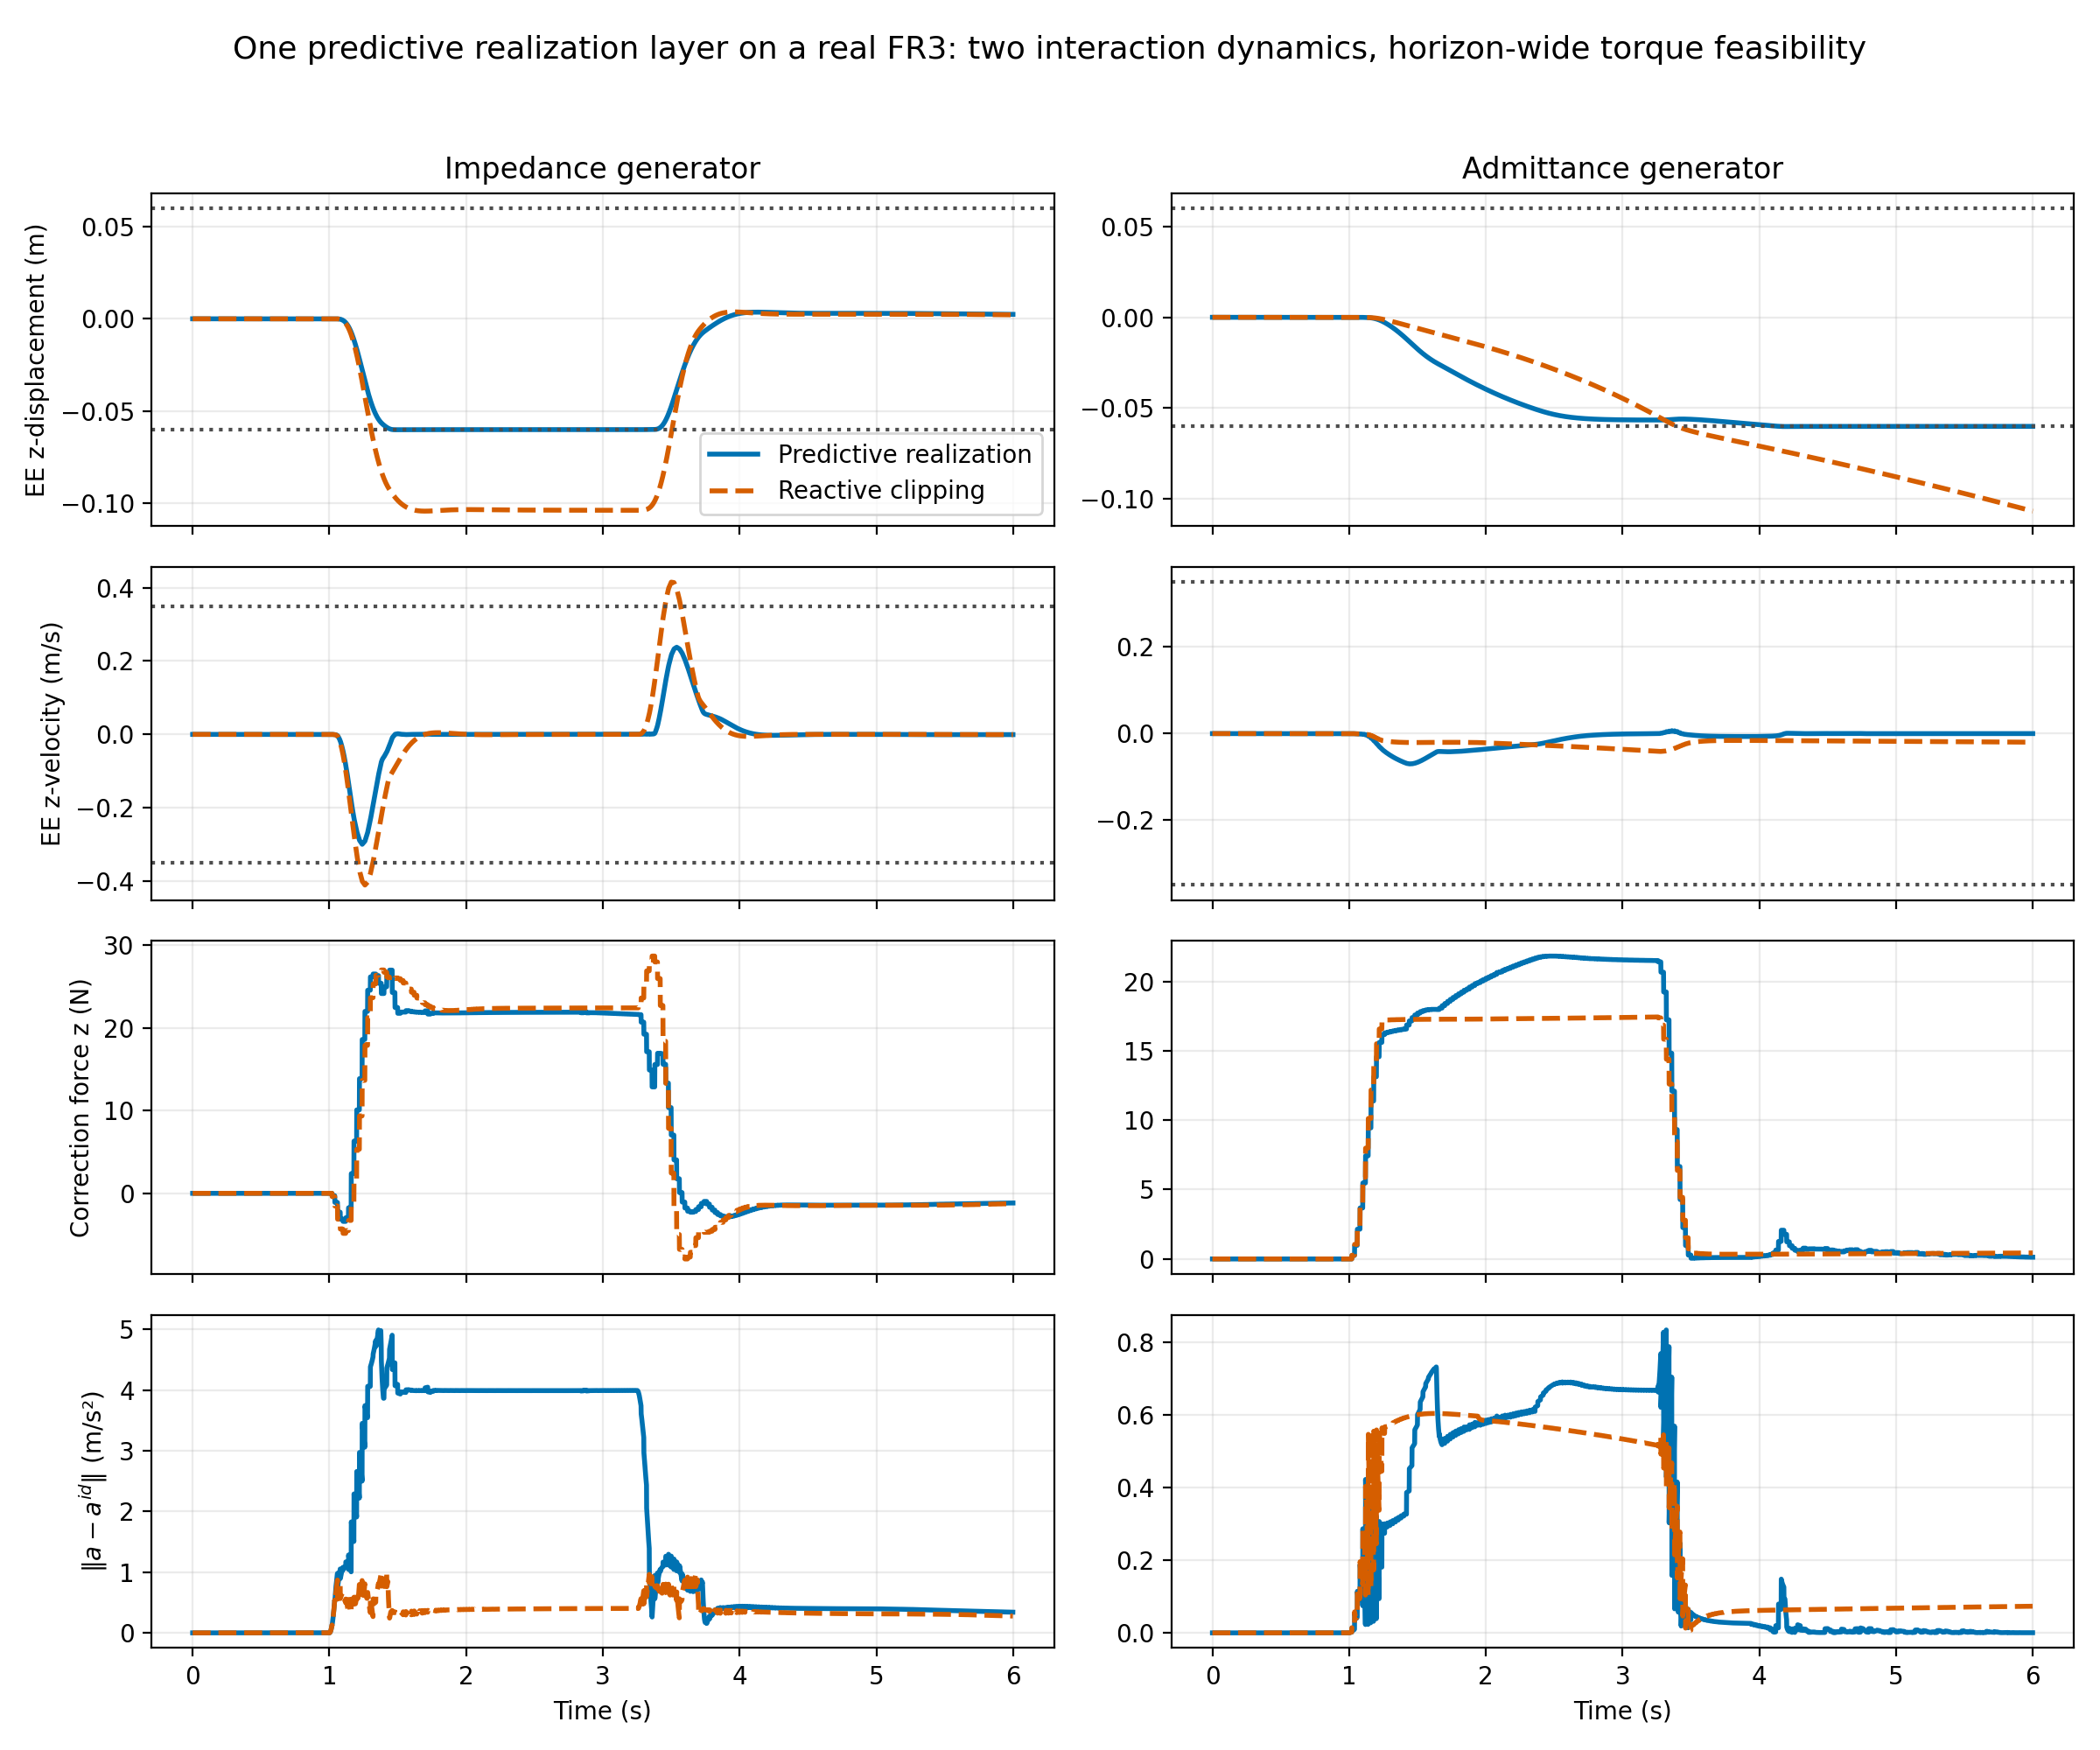
\includegraphics[width=0.95\linewidth]{results/fr3_interaction_dynamics_results.png}
\caption{FR3 基准测试：阻抗（左）与导纳（右），预测式实现（实线）对比不具备预测式工作空间处理能力的指令/速率受限反应式控制器（虚线）。虚线为工作空间/速度界；底行为实测残差；在这一主基准测试中，力矩没有发生截断。预测式实现贴合边界；反应式控制器越界，且对导纳而言从未恢复。}
\label{fig:fr3}
\end{figure}

\begin{table*}[t]
\centering
\caption{FR3 基准测试}
\label{tab:fr3}
\small
\begin{tabular}{@{}llrrrrl@{}}
\toprule
生成器 & 控制器 & RMSE$^{*}$ & 峰值 $|e_z|$ & 峰值速度 & 力矩利用率 & 违反量 \\
& & (m/s$^2$) & (m) & (m/s) & & \\
\midrule
阻抗 & 预测式 & 1.39 / 1.45 & 0.0602 & 0.300 & 37.0\% & 0.0002~m \\
阻抗 & 反应式 & 0.223 / 0.062 & 0.1044 & 0.415 & 37.2\% & 0.0444~m, 0.065~m/s \\
导纳 & 预测式 & 0.212 / 0.290 & 0.0601 & 0.070 & 34.4\% & 0.0001~m \\
导纳 & 反应式 & 0.200 / 0.034 & 0.1066 & 0.041 & 31.7\% & 0.0466~m \\
\bottomrule
\end{tabular}

\vspace{2pt}
\raggedright\footnotesize
$^{*}$残差 RMSE，实测 / 预测。\emph{预测}残差使用第~\ref{sec:fr3-architecture}节的冻结局部模型。\emph{实测}残差则对 1~kHz 的 MuJoCo 末端执行器速度做有限差分，并将该加速度与生成器请求相比较；它是对该仿真非线性被控对象所交付行为的恰当度量。二者之间的差距度量的是局部模型误差与微分误差，因此预测残差不应被解读为一个精确的被控对象残差。与表~\ref{tab:planar}一样，两者都使用按分量计算的 RMSE：全部三个残差分量与全部时间采样点先汇总为一个均值，再开方。这统一了汇总方式，但并不使跨被控对象的数值可以直接作为性能排名。速度按分量报告，以匹配盒约束。最大力矩利用率是最大的比值 $|\tau_j|/\tau_{\max,j}$，这样可以避免比较不可比的 87~N$\cdot$m 与 12~N$\cdot$m 关节限位。预测式方案的求解耗时在下文正文中报告，因为反应式对比方案不求解 QP。
\end{table*}

\begin{table*}[t]
\centering
\caption{FR3 manager 更新残差审计（按分量 RMSE，m/s$^2$）}
\label{tab:fr3-decomposition}
\small
\begin{tabular}{@{}lrrrrrr@{}}
\toprule
生成器 & 模型总量 & $r^{\rm reg}$ & $r^{\rm con}$ & $r^{\rm mod}$ & 实测总量 & 模型闭合误差 \\
\midrule
阻抗  & 1.448 & 0.285 & 1.205 & 0.199 & 1.395 & $<5\!\times\!10^{-16}$ \\
导纳 & 0.283 & 0.0958 & 0.356 & 0.153 & 0.211 & $<3\!\times\!10^{-16}$ \\
\bottomrule
\end{tabular}

\vspace{2pt}
\raggedright\footnotesize
所有列都使用 50~Hz manager 更新时刻的数据；RMSE 各列不需要相加，因为向量项之间可能相互抵消。模型闭合误差是 $r^{\rm model}=r^{\rm reg}+r^{\rm con}$ 中最大的绝对分量误差。随后 $r^{\rm mod}$ 相对有限差分得到的被控对象加速度，闭合了式\eqref{eq:residual-decomposition}。
\end{table*}

在被执行的采样点上，没有任何条件违反逐关节力矩限位，没有任何求解被报告为不可行，且在这一主基准测试中力矩约束从未被触及：最大利用率始终低于 38\%。因此，这一基准测试评测的是在一个工作空间边界处的行为实现，而不是力矩层面的介入。第~\ref{sec:torque-activation}节引入了一个刻意降额的力矩预算压力案例，在其中约束才会被激活。

一项端到端单元测试还收紧了一个关节限位，直到全时域约束被激活。

阻抗参考的无约束静态位移为 $F_h/K_d=20/200=0.10$~m，这本身就已经超过了 0.06~m 的界。反应式截断朝这一平衡点跟踪，峰值达到 0.104~m（略高于静态值，源于与第~\ref{sec:planar-results}节平面情形相同的斜坡超调效应），越界 4.4~cm。预测式实现则在边界被激活期间偏离期望行为加速度，把位移保持在 0.0602~m。

导纳参考没有可比较的平衡位移，只有一个在力被保持期间的稳态速度 $Y F_h=0.01\times20=0.2$~m/s，且没有恢复项能在力释放后把它拉回来。反应式截断在保持期间累积位移，并在力释放后短暂延续，直到速度衰减（时间常数 $T_a=0.3$~s），峰值达到 0.1066~m——4.7~cm 的越界——且从未恢复，因为生成器本身没有位置恢复项（第~\ref{sec:generators}节），而反应式对比方案也没有预见能力来预知边界。预测式实现在到达边界之前就已开始偏离所请求的速度，并保持在 0.0601~m 以内。

表~\ref{tab:fr3-decomposition}避免了把原始 FR3 残差单纯误读为约束介入。对两种生成器而言，在 manager 更新时刻，约束介入都是最大的分量，但有限的正则化项与被控对象/模型项也是实质性的，对导纳条件尤其如此，其中向量相互抵消使得实测总量小于各个分量 RMSE 值。

被部署的 QP 对每个物理状态松弛量 $s$ 都使用精确的变量替换 $z=10^3s$。约束系数使用 $z/10^3$，松弛量的 Hessian 权重变为 $\rho/10^6$，报告的数值再解码为 $s=z/10^3$；因此物理目标函数与可行集保持不变。一项单元测试直接验证了这一矩阵变换。它把浓缩 Hessian 的条件数，对阻抗从 $4.3\times10^9$ 降到 $4.34\times10^3$，对导纳从 $3.8\times10^9$ 降到 $3.77\times10^3$。被部署的 50~Hz 配置还会从上一次的原始/对偶解出发对 OSQP 进行热启动。

一项专门的计时研究（\texttt{run\_fr3\_timing\_study.py}，五次完整的 6~s 重复运行，每个生成器/条件下共 1500 次实际求解）随后测量了完整的 QP 组装与求解耗时。在部署的热启动配置下，阻抗的平均耗时为 3.45~ms，99 分位数为 6.89~ms，最大值为 8.67~ms；导纳分别为 3.68、7.28 与 9.73~ms。因此，在这台开发机器上，全部 3000 次被测量的热启动求解都满足 20~ms 的 manager 周期。匹配的冷启动消融实验平均耗时为 4.24 与 4.02~ms，99 分位数为 7.25 与 8.33~ms，最大值为 17.73 与 14.92~ms；在保存下来的经缩放的表述中，全部 3000 次冷启动求解也都满足 20~ms。因此，热启动被保留下来，是为了额外的裕度，而不是被认定为满足截止时限的唯一手段。

这些墙钟测量是针对被测试机器的证据，而不是一个硬实时或与硬件无关的保证。它们包含 QP 组装与 OSQP，但不包含仅用于残差审计的求解后无约束反事实计算。仿真器同步地调用求解过程，并未实现异步的迟到结果丢弃机制；在不同处理器上部署时，必须重新运行计时测试，若出现超时，则需要显式地保持上一次施加的指令，并拒绝过期的解。

\subsection{力矩激活的运行时介入}
\label{sec:torque-activation}

主基准测试使用标称的 FR3 力矩限制，并未激活它们。为了在不改变行为层的情况下检验运行时介入，我们重复阻抗条件，但把关节 4 的可用预算从其标称的 87~N$\cdot$m 刻意降额到 31.5~N$\cdot$m。这是一次人为构造的执行器预算压力测试，而不是关于 FR3 物理额定值的一个主张。20~N 力剖面、阻抗行为、0.3~s 预测时域、QP 权重、工作空间/速度界，以及 50~Hz 的求解速率，均保持不变。

对比两种预测式运行时。所提出的运行时在全部 15 个预测步上都约束冻结模型下的总力矩。消融方案只在 $i=0$ 处约束同一个力矩；其 QP 维数、行为目标、状态约束与指令/速率界，在其他方面完全相同。

\begin{figure}[t]
\centering
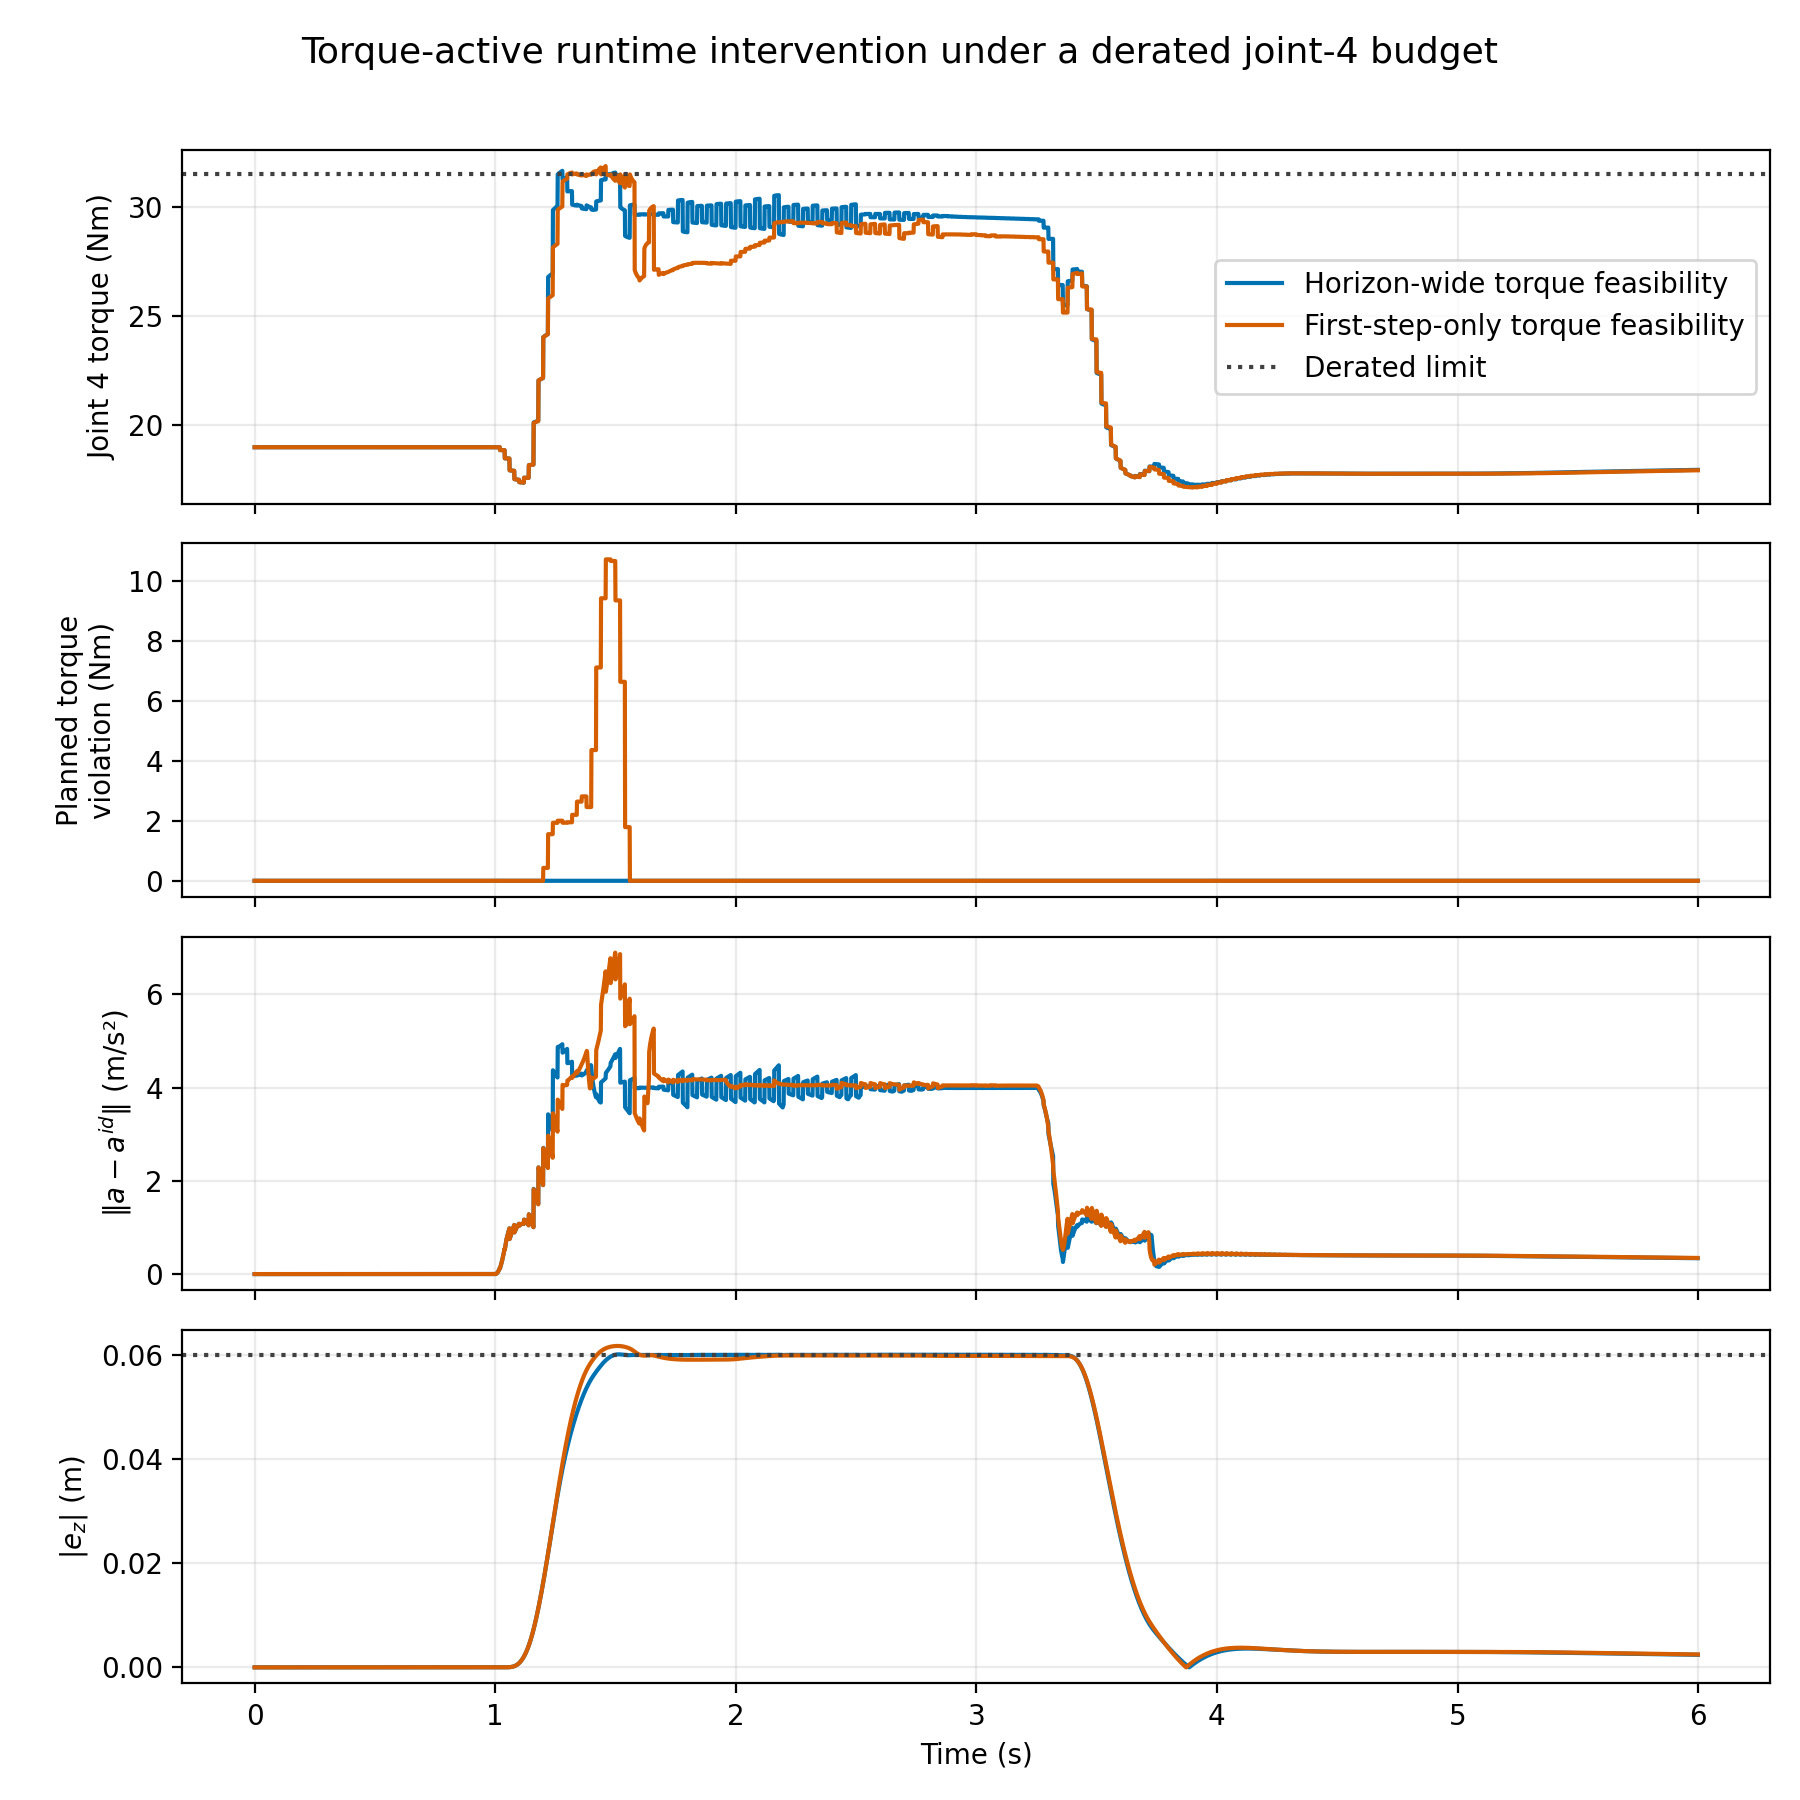
\includegraphics[width=0.95\linewidth]{results/torque_activation_results.png}
\caption{在一个降额的关节 4 预算下的力矩激活介入。全时域强制约束（蓝色）使方案保持可行；仅约束第一步的消融方案（橙色）只满足 $i=0$，并在斜坡期间规划出一个不可行的未来。虚线为降额后的预算与工作空间界。}
\label{fig:torque}
\end{figure}

\begin{table*}[t]
\centering
\caption{力矩激活消融实验}
\label{tab:torque}
\small
\begin{tabular}{@{}lrrrr@{}}
\toprule
强制约束方式 & 计划中违反 & 实际违反 & RMSE$^{*}$ & 峰值 \\
& (N$\cdot$m) & (N$\cdot$m) & (m/s$^2$) & $|e_z|$ (m) \\
\midrule
全部 15 步 & 0.0002 & 0.161 & 1.398 & 0.0603 \\
仅第一步 & 11.329 & 0.380 & 1.466 & 0.0619 \\
\bottomrule
\end{tabular}

\vspace{2pt}
\raggedright\footnotesize
$^{*}$实测残差 RMSE。计划中违反量是相对每个 QP 所使用的冻结模型评估的。全时域方案的数值处于数值求解器容差水平，而仅约束第一步的运行时则会规划出最多超出降额预算 11.329~N$\cdot$m 的未来力矩。被执行采样点的力矩是在 1~kHz 下、从非线性 MuJoCo 状态重新计算得到的；两种情形下都存在的、较小的非零超限，度量的是局部模型的差距，而不是一个被主张的硬性非线性被控对象保证。全时域强制约束缩小了、但没有消除这一失配。该残差使用与表~\ref{tab:planar}和表~\ref{tab:fr3}相同的按分量约定。
\end{table*}

这项实验并不是又一次控制器对比。它检验的是分配给实现运行时的那个架构职责：当一个固定的行为说明与一个执行器预算发生冲突时，运行时会改变指令，通过被暴露出来的行为偏差反映这一点，并避免依赖一个执行器不可行的内部计划。行为层本身保持不变。

\subsection{范围界定与尚待解决的问题}
\label{sec:scope}

这是一次聚焦的架构验证，而不是一次完整的机械臂评估。已实现的行为层仅有阻抗与导纳；场景是一次持续推力，而不是对延迟、传感器噪声或质量失配的扫描；也没有碰撞约束。指令/速率受限的反应式控制器是一个机制层面的消融方案，而不是一个覆盖全面的基线。在线行为层切换的演示（第~\ref{sec:switching}节）仅限于平面情形；一个 FR3 层面的对应实验仍是未来的工作。

人类受试者与硬件验证仍是未来的工作，一个对预测安全滤波器、预测式导纳控制器或 MPIC 基线的忠实匹配实现同样如此。硬件计时与一个显式的过期解处理策略，即便在这台已通过热启动开发机器研究、满足 20~ms 的机器上，也仍需在部署前重新验证。

\section{为何需要行为--实现分离？}
\label{sec:why}

交互行为应当只说明期望的交互动力学；物理可行性应当由机器人独立地实现。第~\ref{sec:intro}节从每一方所依赖的不同变量出发论证了这一点；第~\ref{sec:generators}--\ref{sec:fr3}节则通过一个可执行的仿射实例检验了它。本节针对三种自然的替代方案，直接为这种分离进行辩护。

一种替代方案是联合优化行为与机器人指令。当行为参数本身就是任务决策时，联合优化是恰当的，但分离的做法反而能让一个说明可以被独立地测试与替换，同时把可行性分配给一个稳定的下游契约，其代价是一个固定的行为层，相较于一个完全耦合的设计，可能是次优的。这是一个支持"存在一个有用边界"的论证，而不是一个普遍优越性的主张。

第二种替代方案是直接的机器人 MPC 或轨迹跟踪，它选择指令以最小化一个任务目标，或者相对一个位置/速度参考来评判成功与否。本文的运行时则不同，它接收一个在预测交互状态下求值的律，并度量机器人是否复现了所请求的接触响应，而不生成任何轨迹；MPC 只是当前的实现机制，架构上的选择是优化器接收到什么、以及它报告的是什么样的差异。

第三种替代方案是一个参考调节器，它修改的是一个已设计好的固定控制器上游的参考量。本文的实现层则本身就是指令优化器，其输入是一个期望加速度律，而不是给一个独立内环的设定点。两者都把意图与约束处理分离开来，因此分离本身并不是新颖之处；真正的区别在于接口边界、在线的跨行为替换，以及"期望加速度与实现加速度"的分解方式。

分离具体带来的好处，是可控的可替换性：第~\ref{sec:switching}节在保留实现对象及其携带状态的同时改变了行为层，第~\ref{sec:torque-activation}节在保留行为的同时改变了执行器预算——这是对同一个边界的互补检验，在这个边界上，语义可以改变而无需重建可行性逻辑，可行性也可以介入而无需重写参数。

\section{局限性与尚待解决的理论问题}
\label{sec:limitations}

上述结果在两个被控对象上确立了这一架构上的区分，还不是一个成熟的行为-实现框架所需要的一切。有五个差距值得直白地陈述出来。

第一，已实现的行为类是仿射且无记忆的；一个有状态或学习得到的模型将需要增强的预测机制，以及对模型不确定性的显式处理。

第二，实现代价本身并不意味着无源性——一个无源的参考生成器，可能因为约束引起的偏差或次级优化而被渲染成非无源的。在已实现端口变量上加入一个耗散性约束，配合一个能量 tank 或无源性观测器，是一个自然的扩展方向。

第三，硬性状态约束在一次未预见的冲击之后可能变得不可行（命题~\ref{prop:inheritance}把这标记为一个缺口，而不是一个保证）。FR3 研究通过经松弛处理的工作空间/速度盒约束以及针对求解器不可行情形的反应式后备方案，从操作层面处理了这一点；在被测试的场景中，只有松弛松弛机制被触发，且始终很小。这并不确立一个终端不变集，也没有量化软约束风险，或验证那个从未被触发的后备方案——一个可部署的系统三者都需要。

第四，总实现残差具有物理单位，且依赖于所选择的输出坐标。式~\eqref{eq:residual-decomposition}现在把正则化、约束介入与模型误差区分开来，但并没有把介入量分配到各条具体的约束行上，也没有提供一个归一化的严重程度评分。FR3 研究只涉及平移；姿态由一个固定的 PD 律保持，而不是由一个生成器保持，因此扩展这一接口需要一种有原则的、或按能量加权的跨坐标归一化方式。跨生成器的原始 RMSE 由于尺度不同，并不是一个直接的性能排名，表~\ref{tab:fr3}的实测残差与冻结模型残差在若干条件下存在实质性差异——这是模型充分性与估计差距的证据，而不是对定理~\ref{thm:invariance}的违反。

最后，架构上的新颖性必须相对第~\ref{sec:related}节的全部文献来评估，而不仅仅是相对其最接近的先例。最终最有力的主张，应当建立在已实现的行为层可替换性、形式化的残差保证，以及匹配的实验之上，而不仅仅是术语本身。

\section{结论}

本文的贡献是架构层面的，而不是又一个交互控制器：期望行为说明与受约束的机器人实现，是机器人控制软件中不同的职责，通过一个期望加速度接口，以及一个针对其无记忆仿射子类的预测式实现运行时，被变成了可执行的。平面研究把阻抗替换为导纳、再换回来，同时保留了运行中的实现对象及其指令状态。FR3 研究则相反，它在保留行为层的同时改变了执行器预算：全时域力矩强制约束修改了指令，通过受约束/无约束审计暴露了这一介入，并避免了一个仅约束第一步的消融方案所产生的那种不可行的未来方案。这两者共同检验了这个软件边界的两个方向。这一证据是一个可复现的概念验证，其范围在第~\ref{sec:scope}节与第~\ref{sec:limitations}节中被界定；未来的行为层，无论是基于物理、基于优化，还是学习得到的，只要暴露出一个相容的实现契约，就都可以使用。交互行为应当只说明期望的交互动力学；物理可行性应当由机器人独立地实现。

\section*{可复现性}

全部实验都由固定的、确定性的场景驱动，并由一套配套的测试套件加以验证，该套件端到端地运行每一个脚本化的基准测试，并直接断言其核心主张（力矩限位合规性、求解器可行性、工作空间边界裕度，以及第~\ref{sec:torque-activation}节中全时域方案与仅第一步方案的对比）。它还断言残差分解在平面模型与冻结的 FR3 模型上逐样本闭合，而不是依赖对一张已保存图片的目视检查。物理量（位置、力矩与违反次数）从固定场景出发是逐位可复现的；求解耗时是墙钟时间，只被界定范围，从不被断言为一个精确值。第~\ref{sec:fr3-results}节中关于热启动/Hessian 条件数的求解耗时诊断，由一个独立于主基准测试的专门脚本（\texttt{run\_fr3\_timing\_study.py}）产生，并配有单元测试，用以核查精确的松弛变量矩阵变换、确认热启动收敛到与冷启动相同的指令，并验证重置一个控制器会清除其携带的热启动状态。支撑本文每一幅图与每一张表的代码、配置与已保存的数值制品，均可在项目仓库中获取。

\IEEEtriggeratref{11}
\begin{thebibliography}{99}

\bibitem{ref1}
A. Anand et al., ``Deep Model Predictive Variable Impedance Control,''
arXiv:2209.09614, 2022.

\bibitem{ref2}
K. Haninger, C. Hegeler, and L. Peternel, ``Model Predictive Impedance
Control with Gaussian Processes for Human and Environment Interaction,''
\emph{Robotics and Autonomous Systems}, vol.~165, 104431, 2023.

\bibitem{ref3}
S. Xue et al., ``Model predictive variable impedance control towards
safe robotic interaction in unknown disturbance-rich environments,''
\emph{Robotics and Autonomous Systems}, 2025.

\bibitem{ref4}
M. Sharifi, S. Behzadipour, and G. Vossoughi, ``Nonlinear model
reference adaptive impedance control for human--robot interactions,''
\emph{Control Engineering Practice}, 2014.

\bibitem{ref5}
M. Bednarczyk et al., ``Model Predictive Impedance Control,'' in
\emph{Proc. IEEE Int. Conf. Robotics and Automation (ICRA)}, 2020.

\bibitem{ref6}
T. Gold, A. V\"olz, and K. Graichen, ``Model Predictive Interaction
Control for Robotic Manipulation Tasks,'' \emph{IEEE Trans. Robotics},
2023.

\bibitem{ref7}
M. V. Minniti, R. Grandia, K. F\"ah, F. Farshidian, and M. Hutter,
``Model Predictive Robot-Environment Interaction Control for Mobile
Manipulation Tasks,'' in \emph{Proc. IEEE Int. Conf. Robotics and
Automation (ICRA)}, 2021.

\bibitem{ref8}
E. Garone, S. Di Cairano, and I. Kolmanovsky, ``Reference and command
governors for systems with constraints: A survey on theory and
applications,'' \emph{Automatica}, vol.~75, pp.~306--328, 2017.

\bibitem{ref9}
O. Khatib, ``A Unified Approach for Motion and Force Control of Robot
Manipulators: The Operational Space Formulation,'' \emph{IEEE J.
Robotics and Automation}, vol.~3, no.~1, pp.~43--53, 1987.

\bibitem{ref10}
A. D. Ames, S. Coogan, M. Egerstedt, G. Notomista, K. Sreenath, and
P. Tabuada, ``Control Barrier Functions: Theory and Applications,'' in
\emph{Proc. European Control Conference (ECC)}, 2019.

\bibitem{ref11}
A. Bemporad, M. Morari, V. Dua, and E. N. Pistikopoulos, ``The explicit
linear quadratic regulator for constrained systems,'' \emph{Automatica},
vol.~38, no.~1, pp.~3--20, 2002.

\bibitem{ref12}
P. Tondel, T. A. Johansen, and A. Bemporad, ``An algorithm for
multi-parametric quadratic programming and explicit MPC solutions,''
\emph{Automatica}, vol.~39, no.~3, pp.~489--497, 2003.

\bibitem{ref13}
K. P. Wabersich and M. N. Zeilinger, ``A predictive safety filter for
learning-based control of constrained nonlinear dynamical systems,''
\emph{Automatica}, vol.~129, Art.~no.~109597, 2021.

\bibitem{ref14}
A. Alharbat, H. Esmaeeli, D. Bicego, A. Mersha, and A. Franchi,
``Three fundamental paradigms for aerial physical interaction using
nonlinear model predictive control,'' in \emph{Proc. Int. Conf. Unmanned
Aircraft Systems (ICUAS)}, 2022, pp.~39--48.

\bibitem{ref15}
A. Alharbat, C. Gabellieri, A. Mersha, and A. Franchi, ``Predictive
admittance control for aerial physical interaction,'' \emph{IEEE Robot.
Autom. Lett.}, vol.~10, no.~11, pp.~11235--11242, 2025.

\bibitem{ref16}
Q. Leboutet, E. Dean-Leon, F. Bergner, and G. Cheng, ``Tactile-based
whole-body compliance with force propagation for mobile manipulators,''
\emph{IEEE Trans. Robotics}, vol.~35, no.~2, pp.~330--342, 2019.

\bibitem{ref17}
S. S. Kumbhar, A. M. Kulkarni, and P. Artemiadis, ``Efficient and
compliant control framework for versatile human--humanoid collaborative
transportation,'' arXiv:2512.07819, 2025.

\bibitem{ref18}
F. Lawan, X. Han, J. Carrasco, B. Lennox, and X. Cheng,
``Safety-critical adaptive impedance control via nonsmooth control
barrier functions under state and input constraints,'' arXiv:2605.28367,
2026.

\bibitem{ref19}
A. Del Prete, F. Nori, G. Metta, and L. Natale, ``Prioritized
motion--force control of constrained fully-actuated robots: Task Space
Inverse Dynamics,'' \emph{Robotics and Autonomous Systems}, 2014,
doi: 10.1016/j.robot.2014.08.016.

\bibitem{ref20}
J. Lee, S. H. Bang, E. Bakolas, and L. Sentis, ``MPC-based hierarchical
task space control of underactuated and constrained robots for execution
of multiple tasks,'' arXiv:2009.05891, 2020.

\end{thebibliography}

\end{document}
